\documentclass[11pt,a4paper,UKenglish]{memoir}
% Template by DTU LaTeX support group, v20090423

\usepackage[utf8]{inputenc} % Must correspond to the input encoding used by the editor
\usepackage{babel} % Other languages, in this case UKenglish
\usepackage[T1]{fontenc} % font encoding (output), use T1 for most latin languages
\usepackage{lmodern} % vector based Computer Modern font
\usepackage{graphicx} % for graphics

\usepackage{caption}
\usepackage{subcaption}

\graphicspath{{./figures/}} % path to figures and images

\usepackage{mathtools} % mathmatics

\usepackage{xcolor}
\usepackage[plainpages=false,pdfpagelabels,pageanchor=false]{hyperref} % active links
\hypersetup{%
  pdfauthor={
  	Dzitkowski Karol \\
	Marco Becattini},
  pdftitle={02450 Project 3},
  pdfsubject={Introduction to Machine Learning and Data Mining},
  citebordercolor={0 1 0}, % The color of the box around citations (change to 1 1 1 to remove)
  linkbordercolor={1 0 0}, % The color of the box around normal links
  pagebordercolor={1 1 0}, % The color of the box around links to pages
  urlbordercolor= {1 1 1}  % The color of the box around links to URLs
}
\usepackage{memhfixc}% fixes for hyperref

% The following can be used if not using custom frontpage
\title{02450 Project 3}
\author{
	Dzitkowski Karol \\
	Marco Becattini
}
\date{\today}%

% \includeonly{preface,testing} % Only compile those files you are working in (to save compile time, and power)

\begin{document}
\frontmatter % roman page numbering
%\maketitle  % use this if not using custom frontpage


\begin{titlingpage}
\centering \parindent=0pt
\newcommand{\HRule}{\rule{\textwidth}{1mm}}
\vspace*{\stretch{1}} \HRule\\[1cm]\Huge\bfseries
02450 Project 2\\[0.7cm]
\large Report\\[1cm]
\HRule\\[4cm]  
\large by Karol Dzitkowski\\
Marco Becattini\\
\vspace*{\stretch{2}} \normalsize %
\begin{flushleft}
Technical University of Denmark\\
Department of Applied Mathematics and Computer Science\\
Introduction to Machine Learning and Data Mining\\
Tue Herlau\\
\today \end{flushleft}
\end{titlingpage}


\begin{abstract}
This is the abstract.
\end{abstract}


%\tableofcontents
%\listoffigures
%\listoftables

\mainmatter % arabic page numbering

\chapter*{Clustering}
We clustered our data containing letters with a set of their attributes using
Gaussian Mixture Model as well as with Hierarchical clustering. We used
cross-validation to estimate the optimal parameters for both algorithms. At
the end we estimated the quality of both algorithms in terms of our true labels
which are letters.


\section{Gaussian Mixture Model (GMM)}
For GMM algorithm we used double cross-validation to estimate the best number of
components in internal loop and calculating quality score in external loop as
an average of scores. We also applied Principal Component Analysis to visualize
the results in more human friendly way. We used only a subset of our dataset for
performance reasons, using random sampling. We can see the results in the figure
\ref{fig:GMM}
\begin{figure}[!tbh]
  \centering
  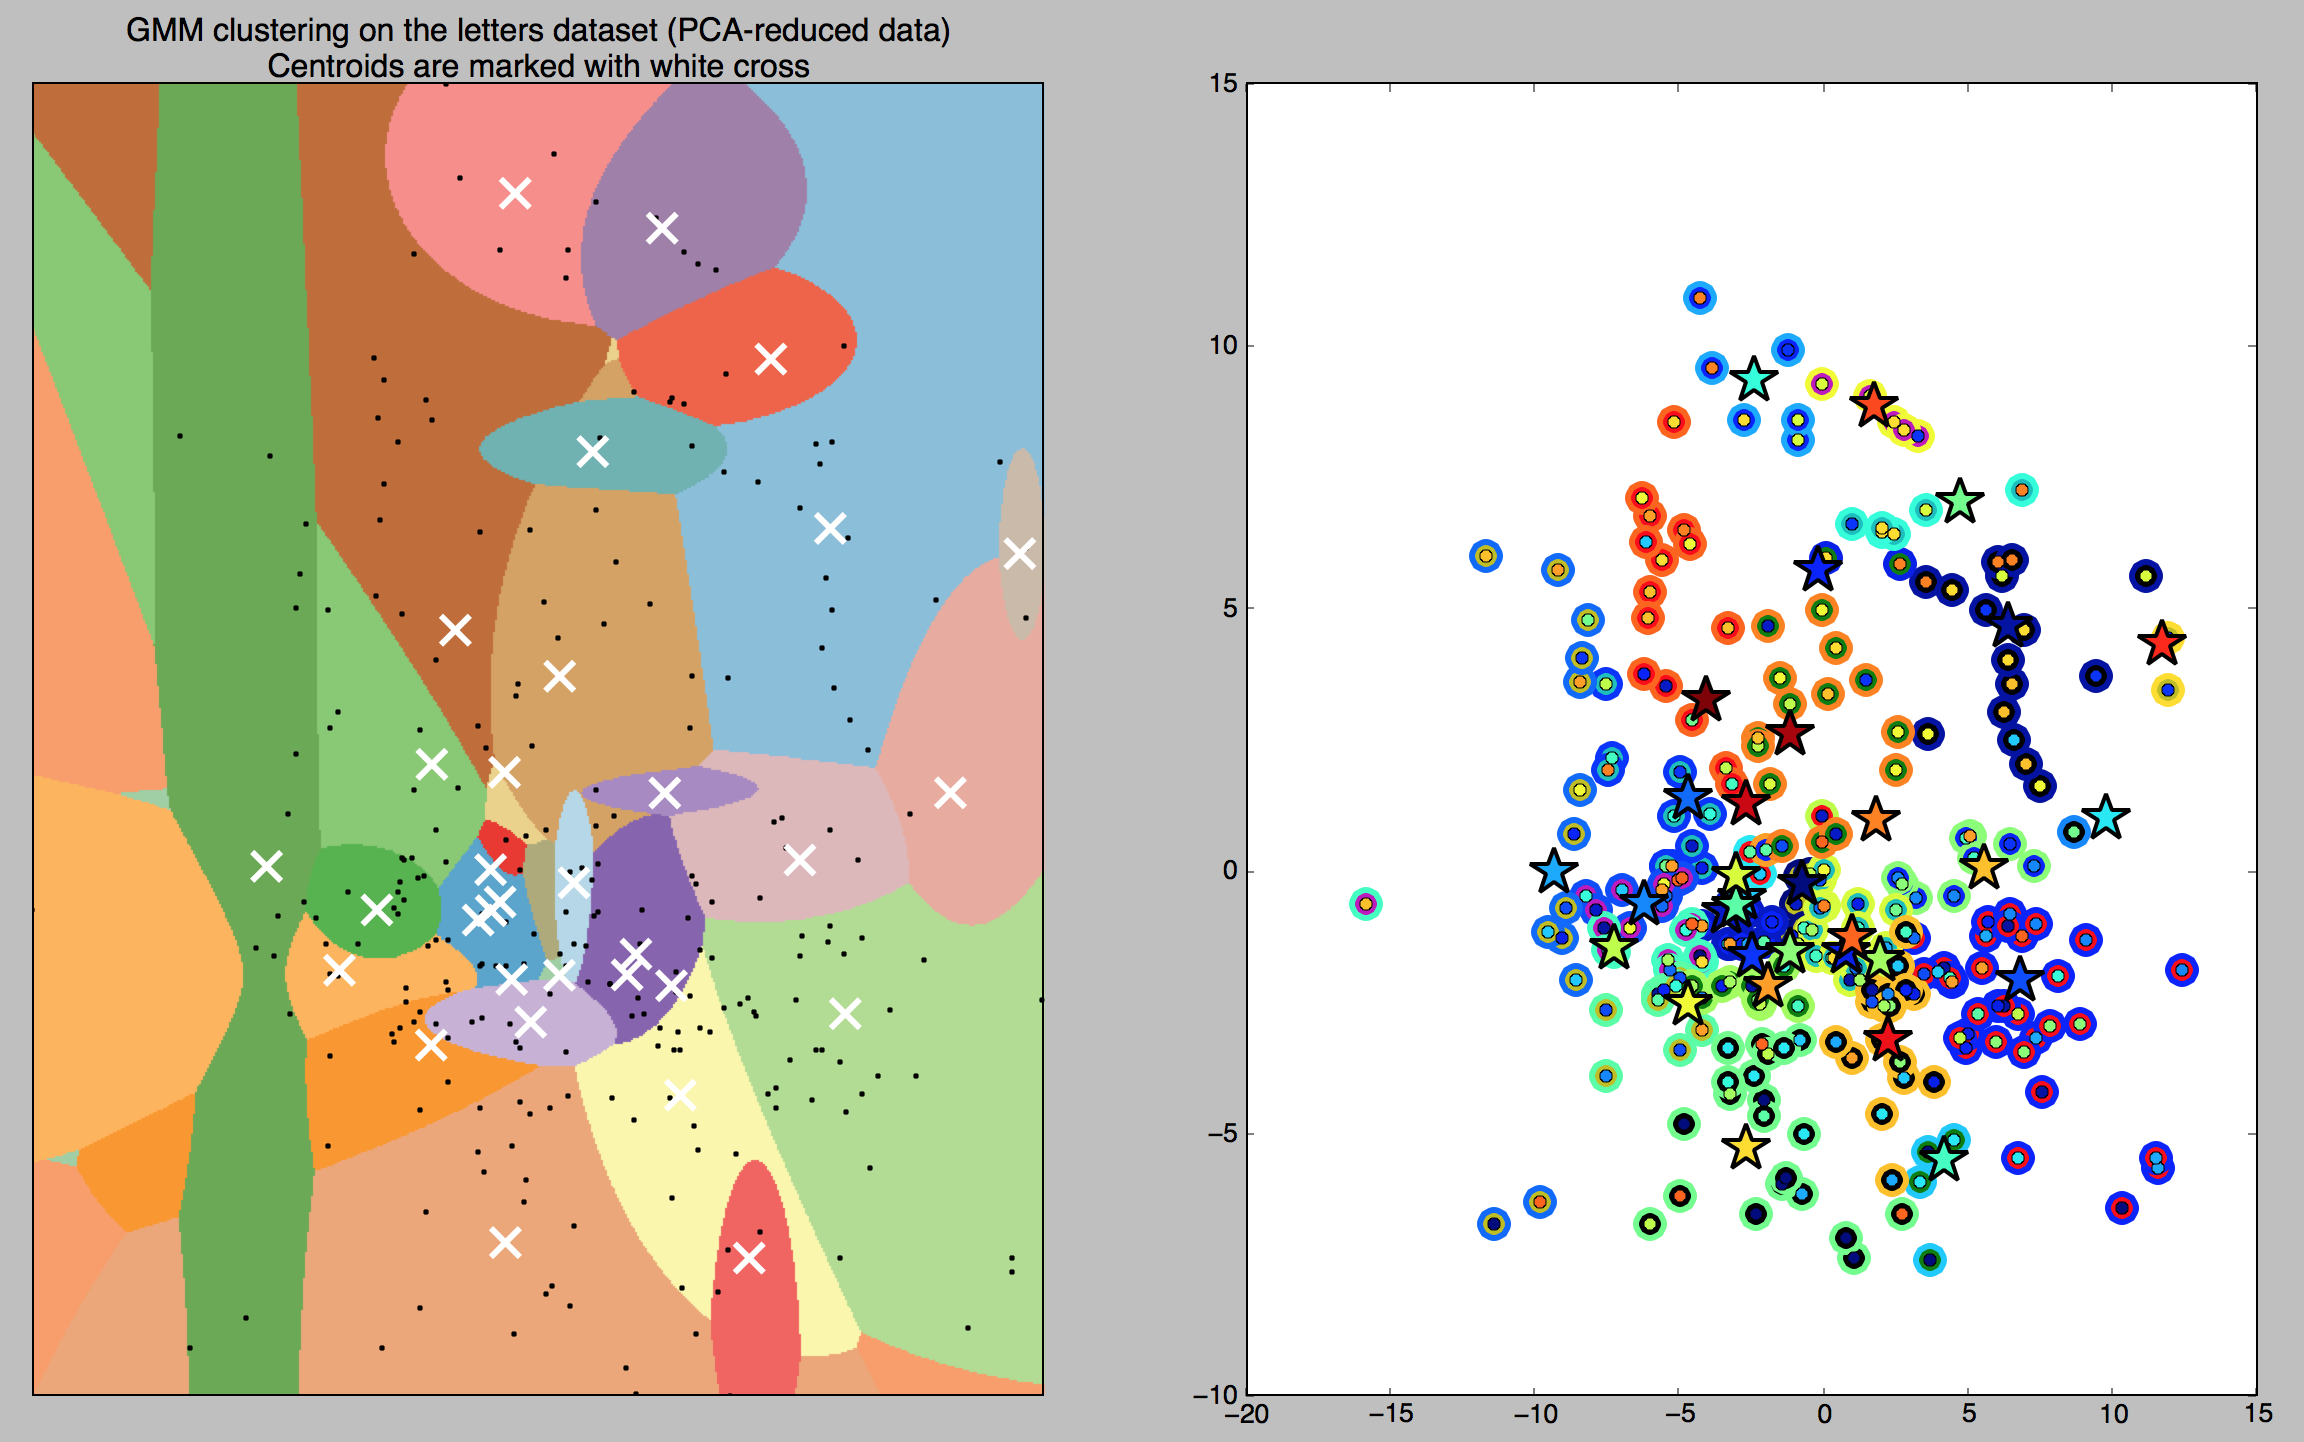
\includegraphics[width=0.6\textwidth]{figures/GMM_pca_2_2}
  \caption{GMM - clustered (data reduced using PCA)}
  \label{fig:GMM}
\end{figure}
In an average the most optimal number of components choosed in internal
cross-validation loop was 30. Which is a close to the number of actual classes.
We can see how the quality of GMM clustering in terms of actual labels depends
on the number of components in the figure \ref{fig:ami}
\begin{figure}[!tbh]
  \centering
  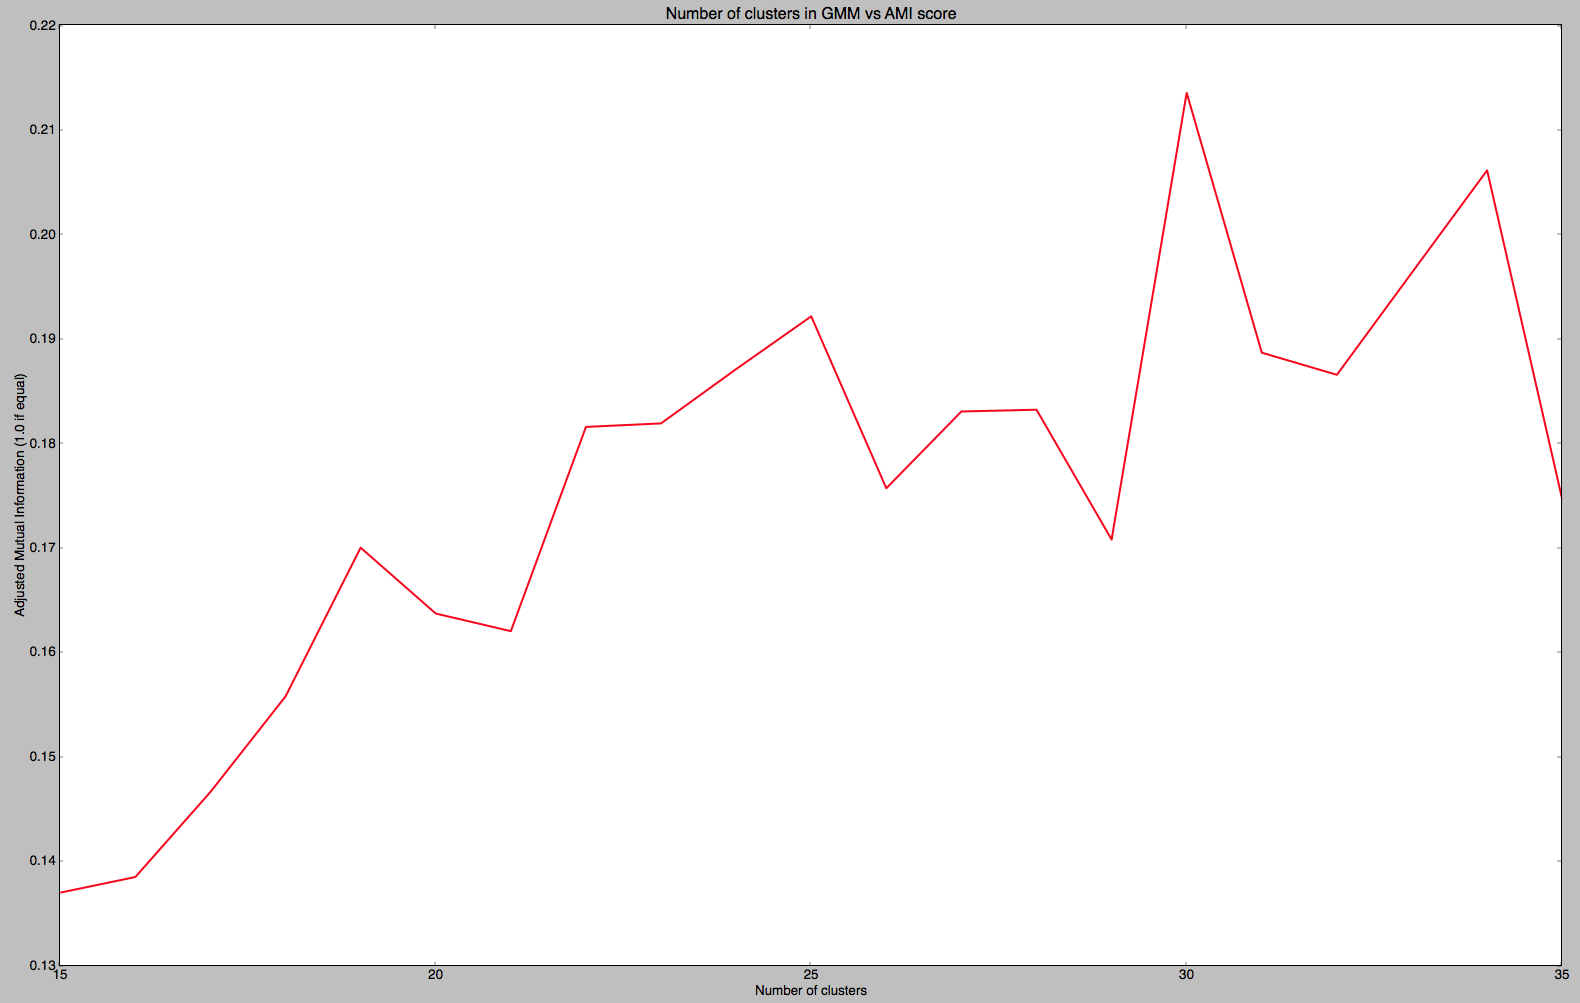
\includegraphics[width=0.6\textwidth]{figures/ami}
  \caption{GMM - quality vs components count}
  \label{fig:ami}
\end{figure}
Cluster centers should be in ideal case (especially if we consider number of
components equal to the number of actual classes - 26) an average vector from
the attribute vectors corresponding to particular letters. So the centroids
should correspond to some ,,unified'' letters.

\section{Hierarchical Clustering}
We also used single cross-validation technique in Hierarchical Clustering and
choose the best metric and linkage function from all available options. Score
results are mesured for best performing option sets. We also used PCA to help
visualize results (Figure~\ref{fig:hier_all} and Figure~\ref{fig:hier_pca}).
\begin{figure}[!tbh]
  \centering
  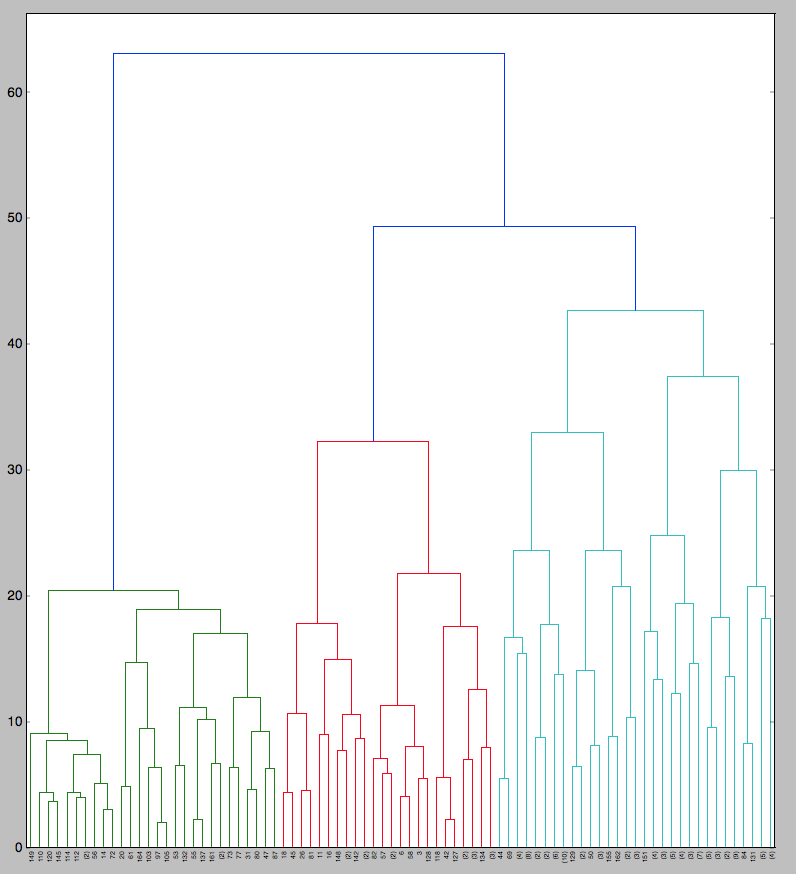
\includegraphics[width=0.6\textwidth]{figures/Hier_all_1}
  \caption{Hierarchical clustering (without PCA reduction)}
  \label{fig:hier_all}
\end{figure}
\begin{figure}[!tbh]
  \centering
  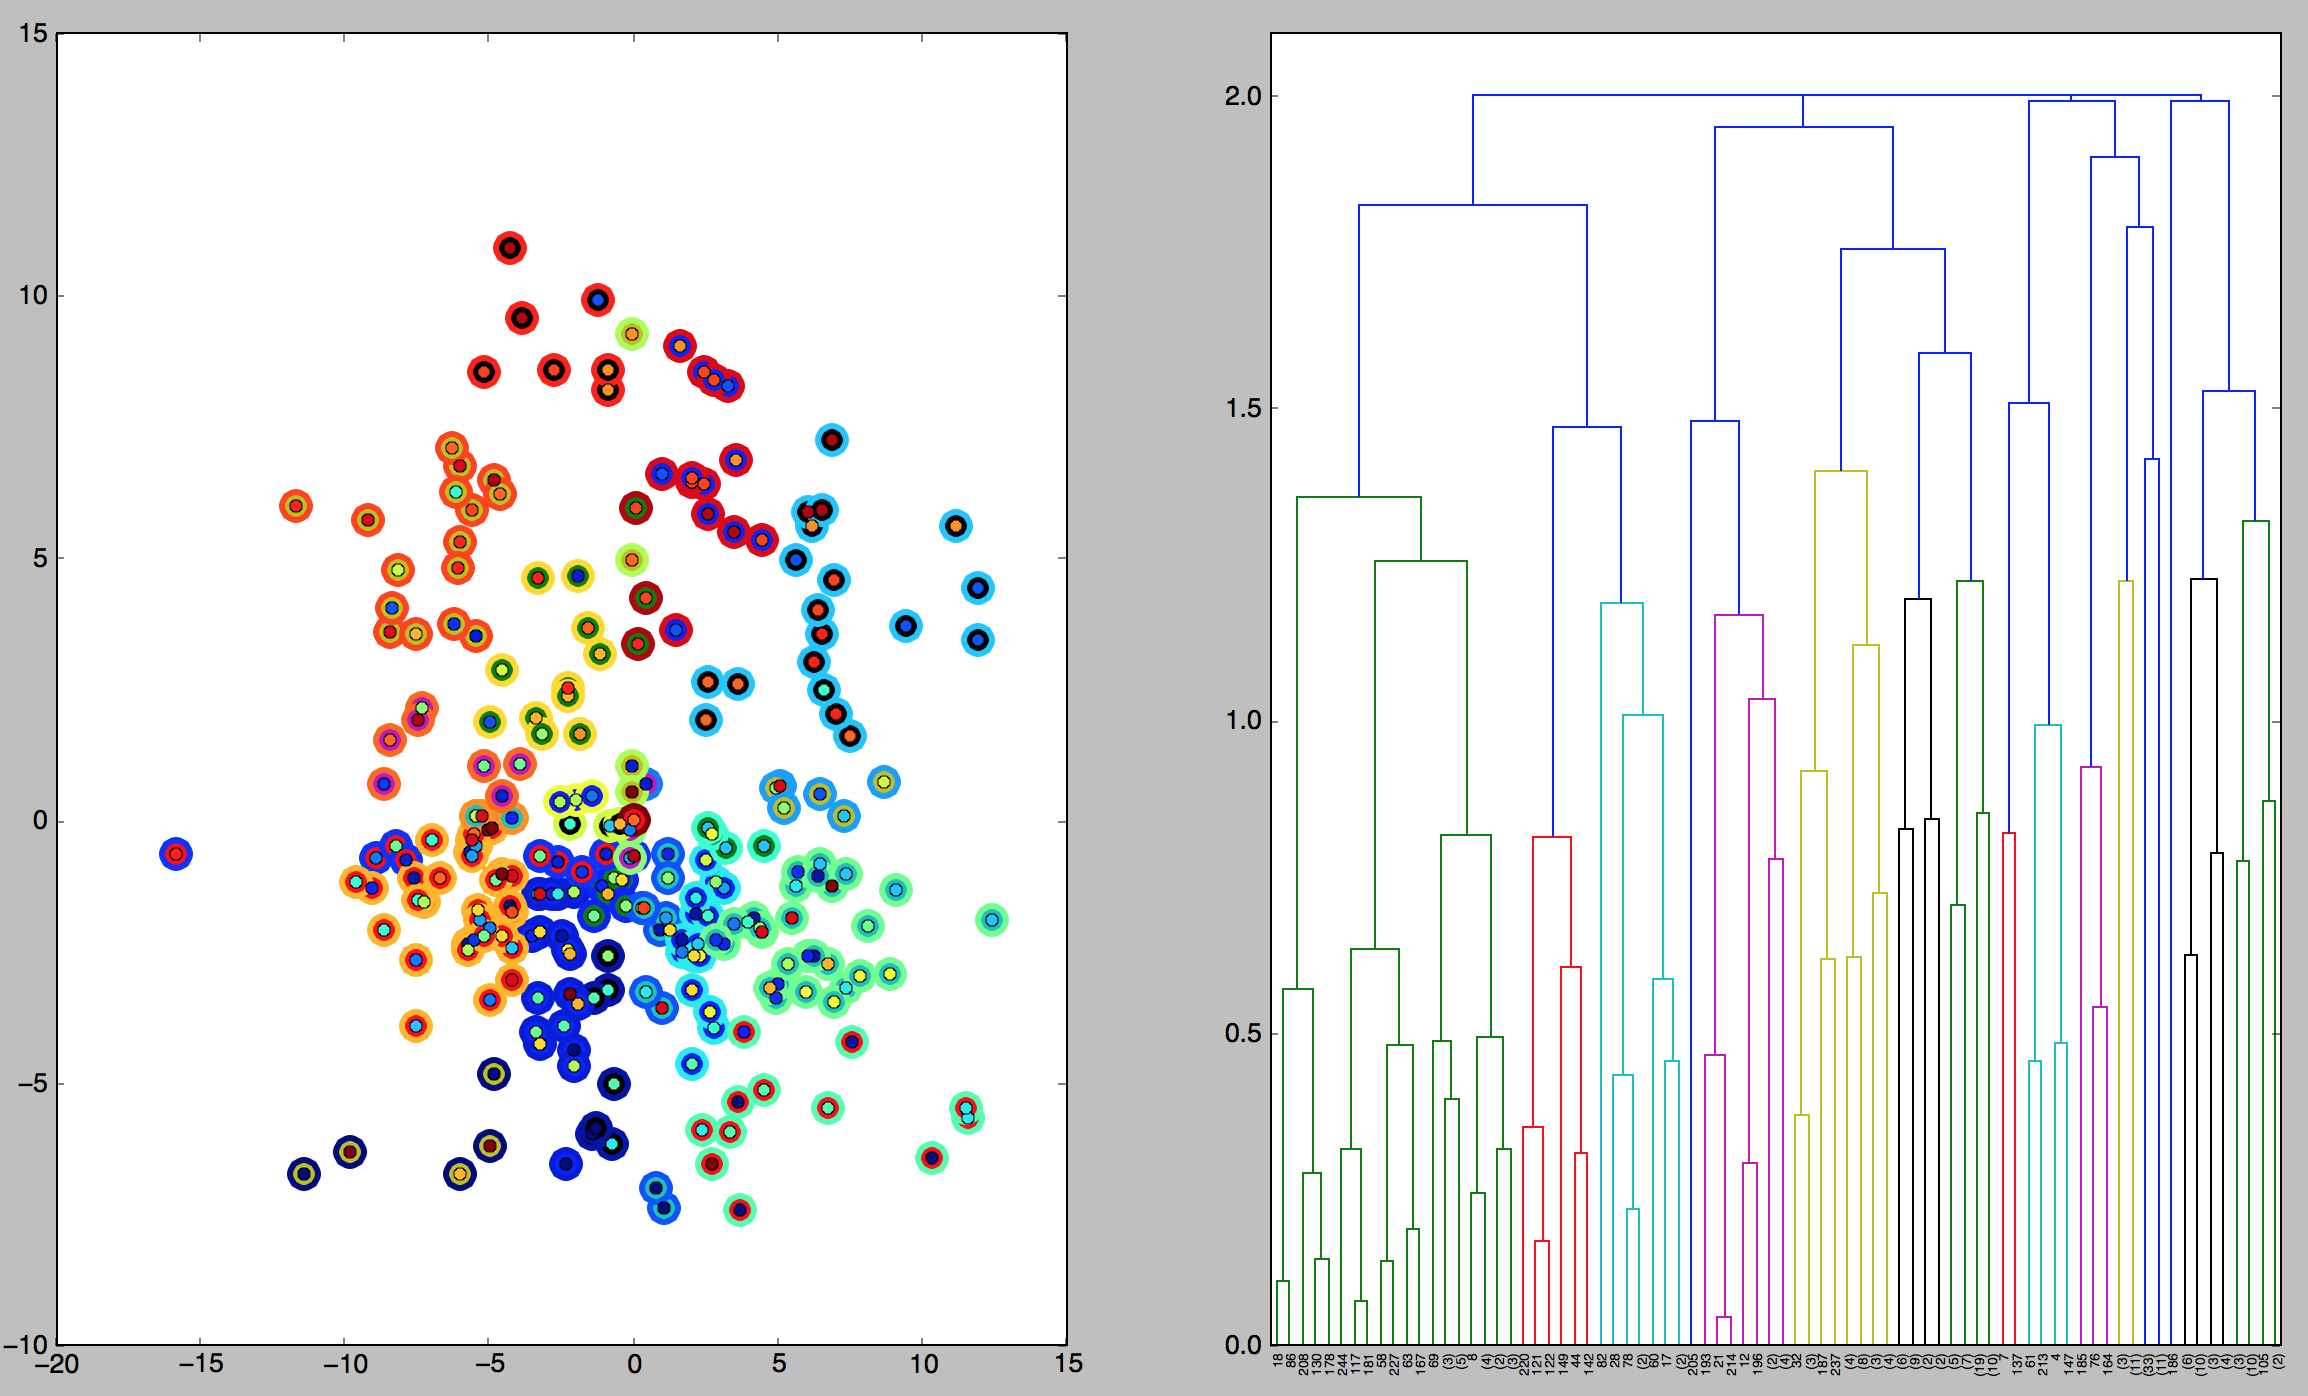
\includegraphics[width=0.6\textwidth]{figures/Hier_pca_2_1}
  \caption{Hierarchical clustering (data reduced using PCA)}
  \label{fig:hier_pca}
\end{figure}
Even using first two principal components explaining the most variance, results
are dyrastically worse than when we use all data dimensions. The most commonly
choosed options by the program were ('ward', 'euclidean') which means that the
ward linkage function and euclidean metric were most suitable for our data.

\section{Evaluation}
We choosed an adjusted mutual info score metric as our quality messure for
clustering methods. For two clusterings U and V, the AMI is given as:
$$ AMI(U, V) = [MI(U, V) - E(MI(U, V))] / [max(H(U), H(V)) - E(MI(U, V))] $$
And has following properties:
\begin{enumerate}
\item Perfect labeling is scored 1.0
\item Independent labelings have non-positive scores
\item No assumption is made on the cluster structure
\item It is symmetric
\item It is independent of the absolute values of the labels: a permutation of
      the class or cluster label values won’t change the score value in any way
\item It accounts for the fact that the MI is generally higher for two
      clusterings with a larger number of clusters, regardless of whether there
      is actually more information shared
\end{enumerate}

Reaserch has shown that Hierarchical clustering performs better for our data
than GMM and also that both methods have better scores while having more data.
However it was impossible for performance reasons to run this methods on more
than 3000 records of our data, where results would be even better. It is
visualized in the figure \ref{fig:scores}
\begin{figure}[!tbh]
  \centering
  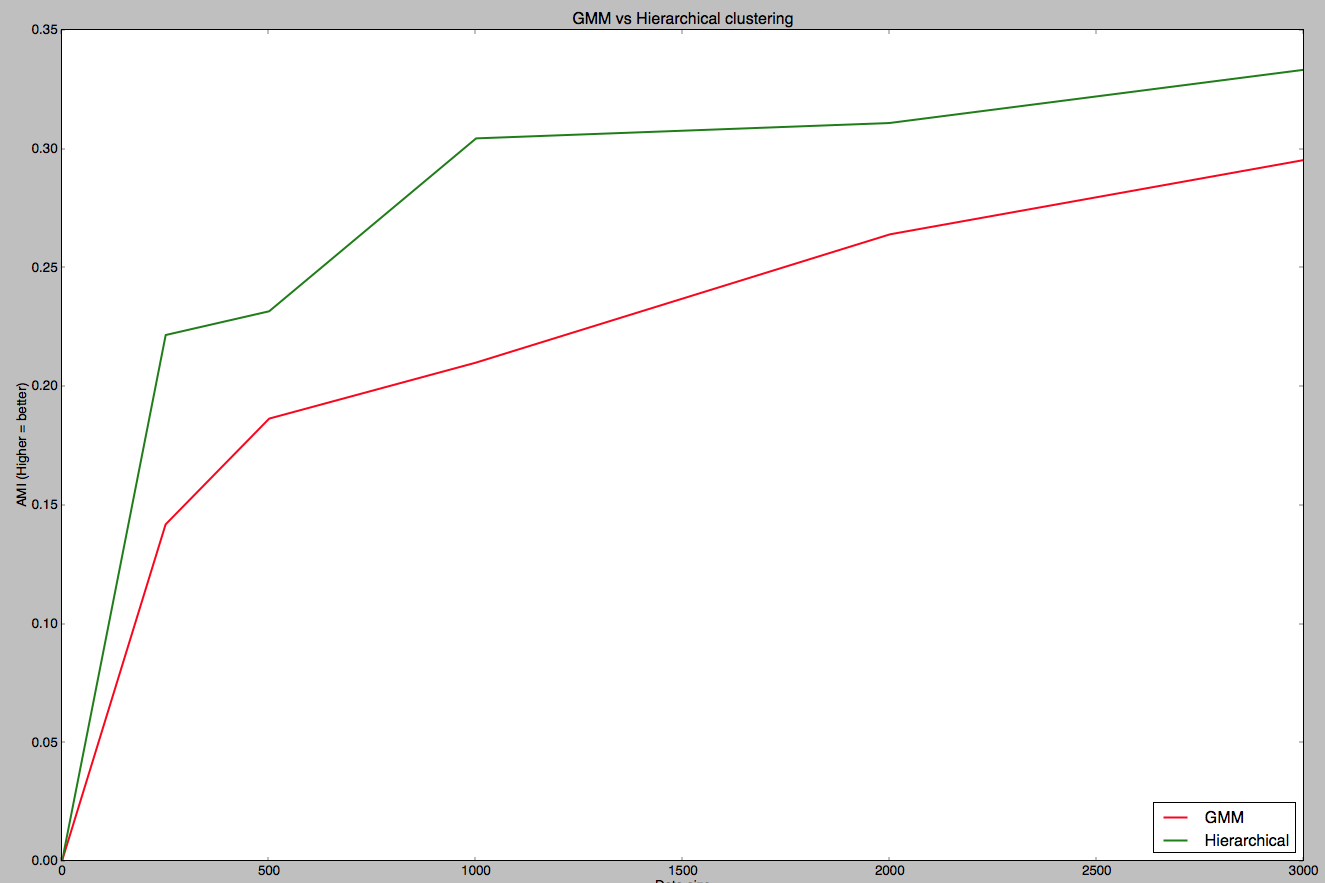
\includegraphics[width=0.6\textwidth]{figures/scores}
  \caption{GMM vs Hierarchical clustering quality}
  \label{fig:scores}
\end{figure}

%In this report we apply regression and classification to the "Letter Image Recognition" dataset
\chapter*{Outlier / Anomaly detection}
\setcounter{chapter}{3}

In statistics, an outlier is an observation point that is distant from other observations. For this reason we apply outlier / anomaly detection for each class of our dataset in order to consider which data for each class could be excluded from the data set.
Below is shown an example of outlier detection applied to the subset that correspond to the letter `A'.
We calculate for all the samples the leave-one-out Gaussian Kernel density, KNN density, KNN average relative density and distance to K-th nearest neighbor for with K=5.\\
For each of the metrics, we sort the outlier scores and inspect their distribution. We set an outlier threshold where there is a significant ``jump'' in the scores, in order to have around 35 outliers (about 5\% of the total samples). We consider only the outliers which are detected by all four methods, and in this way we obtain 4 outliers (about 0.5\% of the samples).
In the bottom table are specified our results:
\begin{center}
    \begin{tabular}{ | p{3cm} | p{9cm} |}
    \hline
    \textbf{Method}  & \textbf{Selected outliers (indices)} \\ 
    \hline
    Gaussian Kernel density & [
   495
   741
   311
   133
   159
    51
    18
   399
    86
   739
   136
   566
   515
   423
     2
   227
   760
   285
   489
   152
   149
   572
   655
   688
   469
   114
   124
   762
   130
   638
   327
   645
   307 ]\\ 
    \hline
    KNN density & [ 18
   311
   495
   741
   133
   159
   515
    86
   399
    51
   739
   136
   489
   566
   285
   116
   688
   760
   227
   152
   423
   500
   469
   114
   655
     2
   149
   657
   504
   696
   238
   604
   572
   439
   124 ] \\ 
    \hline
    KNN average relative density & [ 197
   156
   102
   215
   356
    31
   399
   217
   127
   573
   701
   617
   124
   355
   530
    86
    36
   304
   450
   184
   133
   452
   321
   183
   746
   728
   714
   724
   638
   627
   285
   149 ]\\ 
    \hline
    Distance to 5th nearest neighbor & [     18
   311
   116
   515
   741
   399
   439
   500
    86
   133
   230
   495
   739
   159
   292
   489
   657
    51
   132
   136
   152
   238
   284
   285
   390
   438
   604
   688
    57
   114
   212
   227
   504
   566
   655
   696 ]\\ 
    \hline
    Common to all method & [ 51    86   739   688 ]\\ 
    \hline
    \end{tabular}
\end{center}

In figure  \ref{fig:r1} we represent one bar plot for each metrics. Each column is a pattern and the y-axis is the outlier score density (or distance for for 5th nearest neighbor ).  Red columns are patterns with lower outlier score (or highest for 5th nearest neighbor) that we decided to set as otliers.

\begin{figure}[htbp]
        \center
       	\begin{subfigure}[b]{0.46\textwidth}
                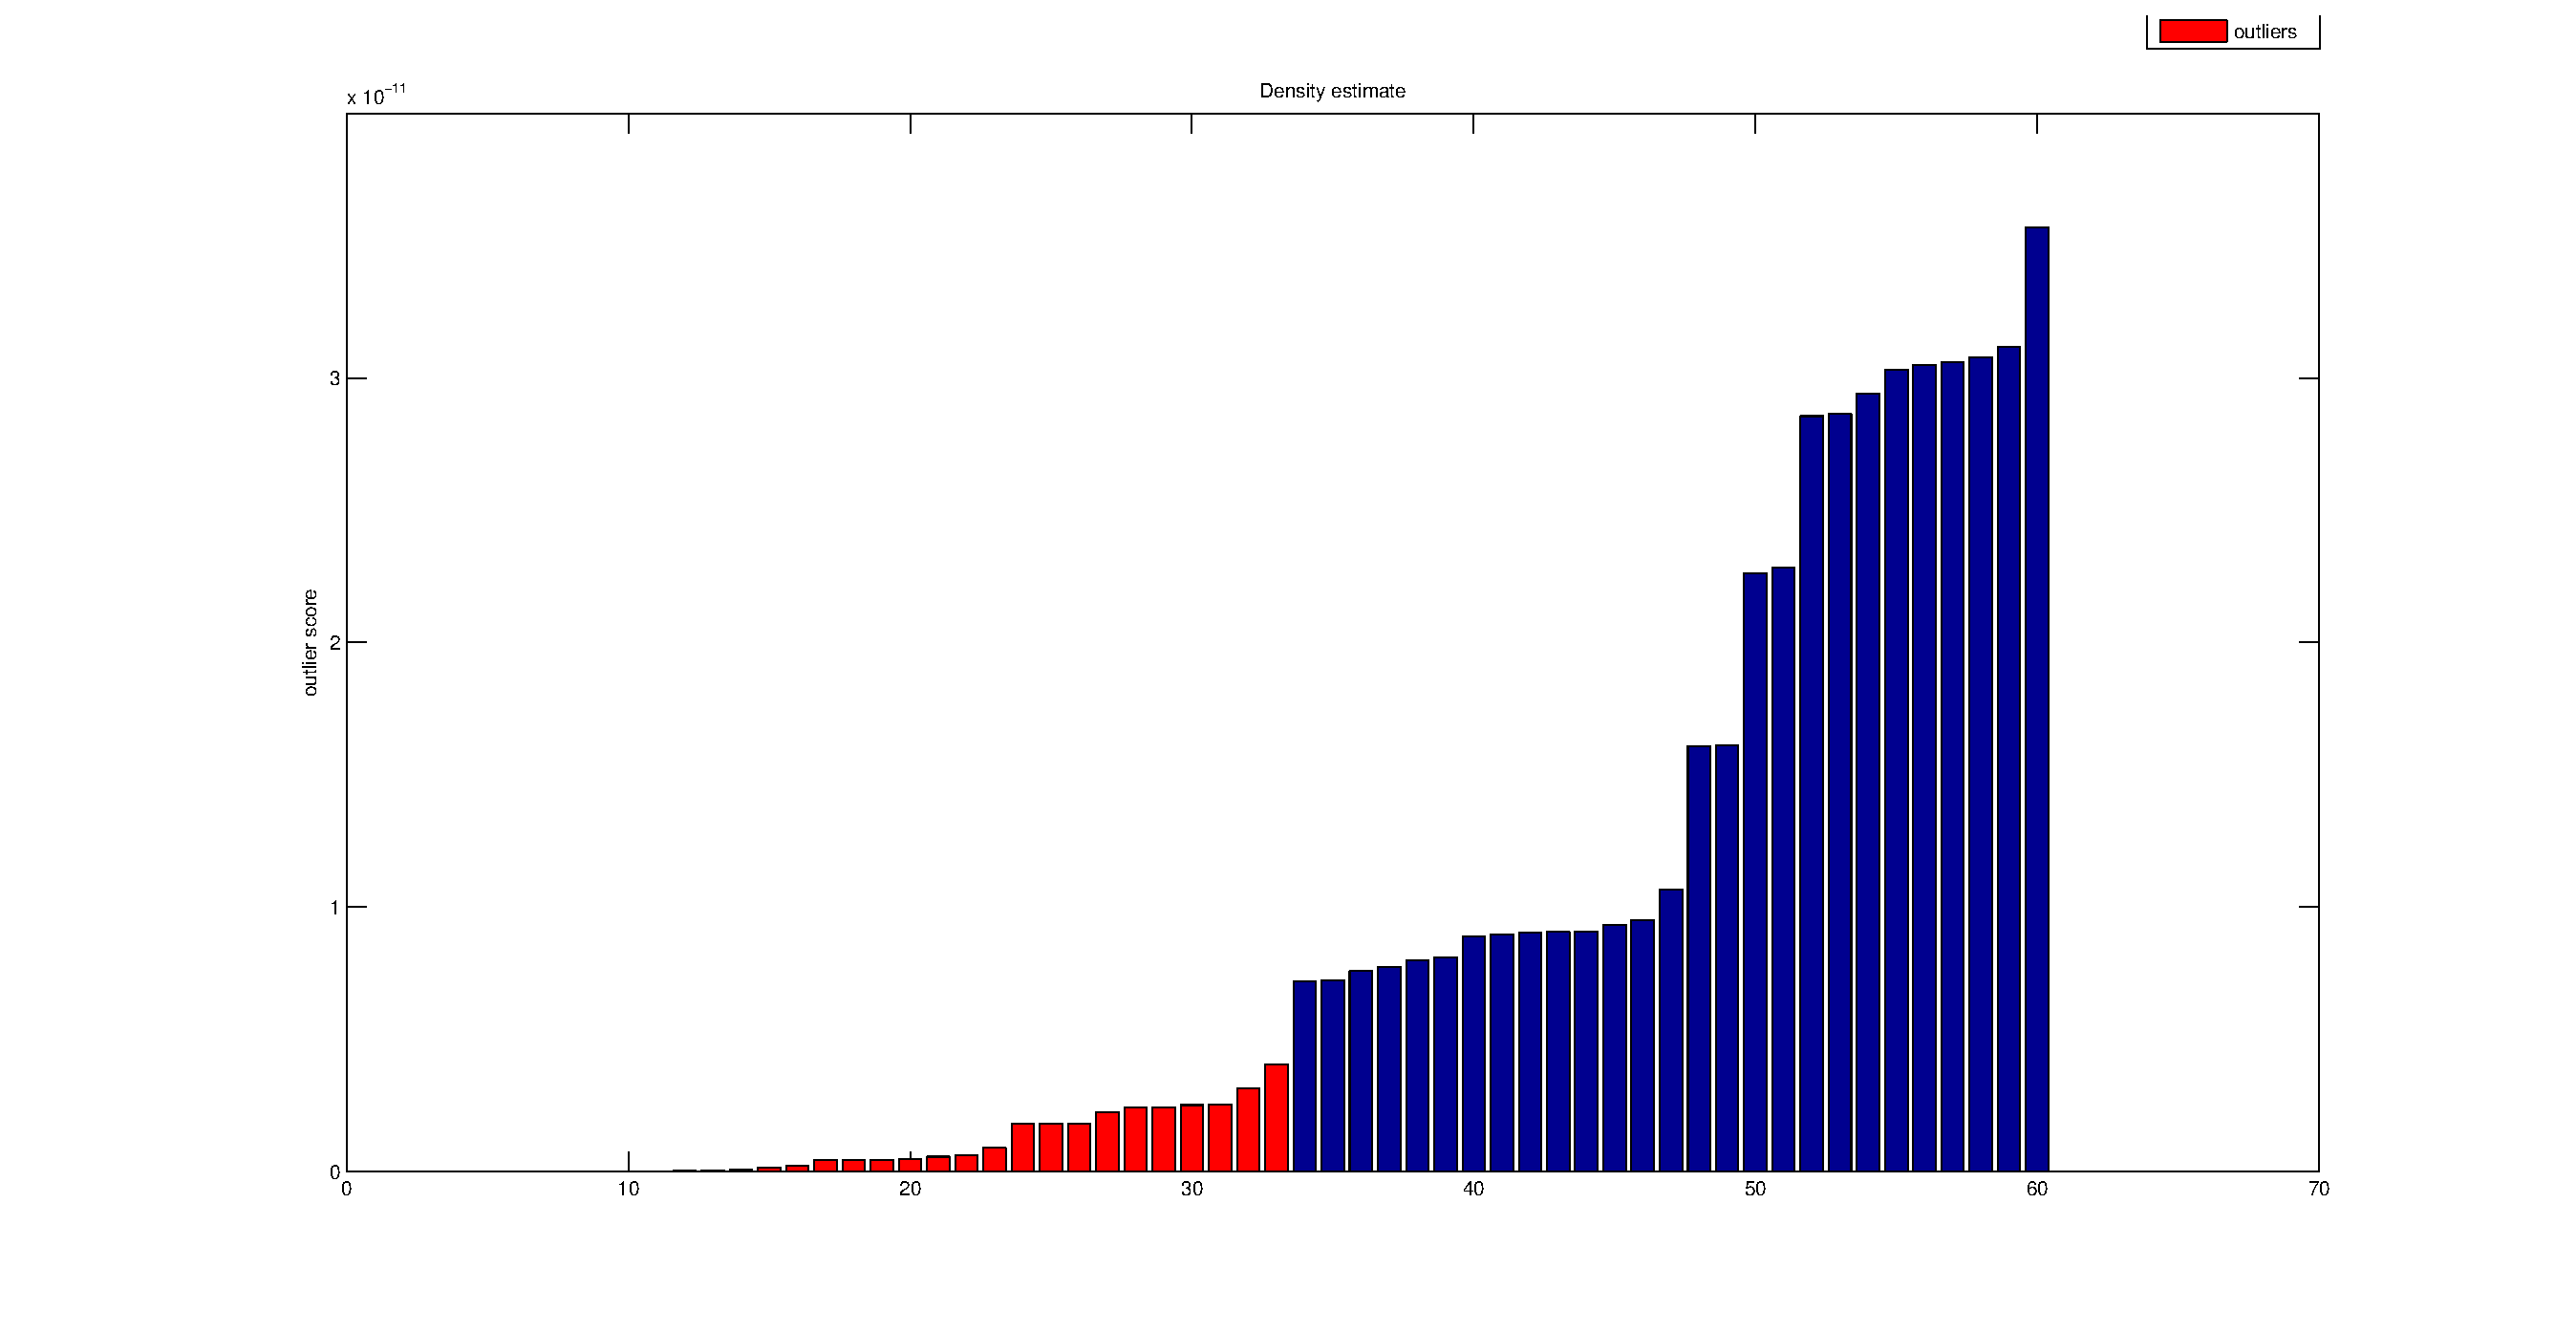
\includegraphics[width=7.4cm]{figures/01.eps}
                \caption{Density estimate outliers}
        \end{subfigure}%
        \qquad
        \begin{subfigure}[b]{0.46\textwidth}
                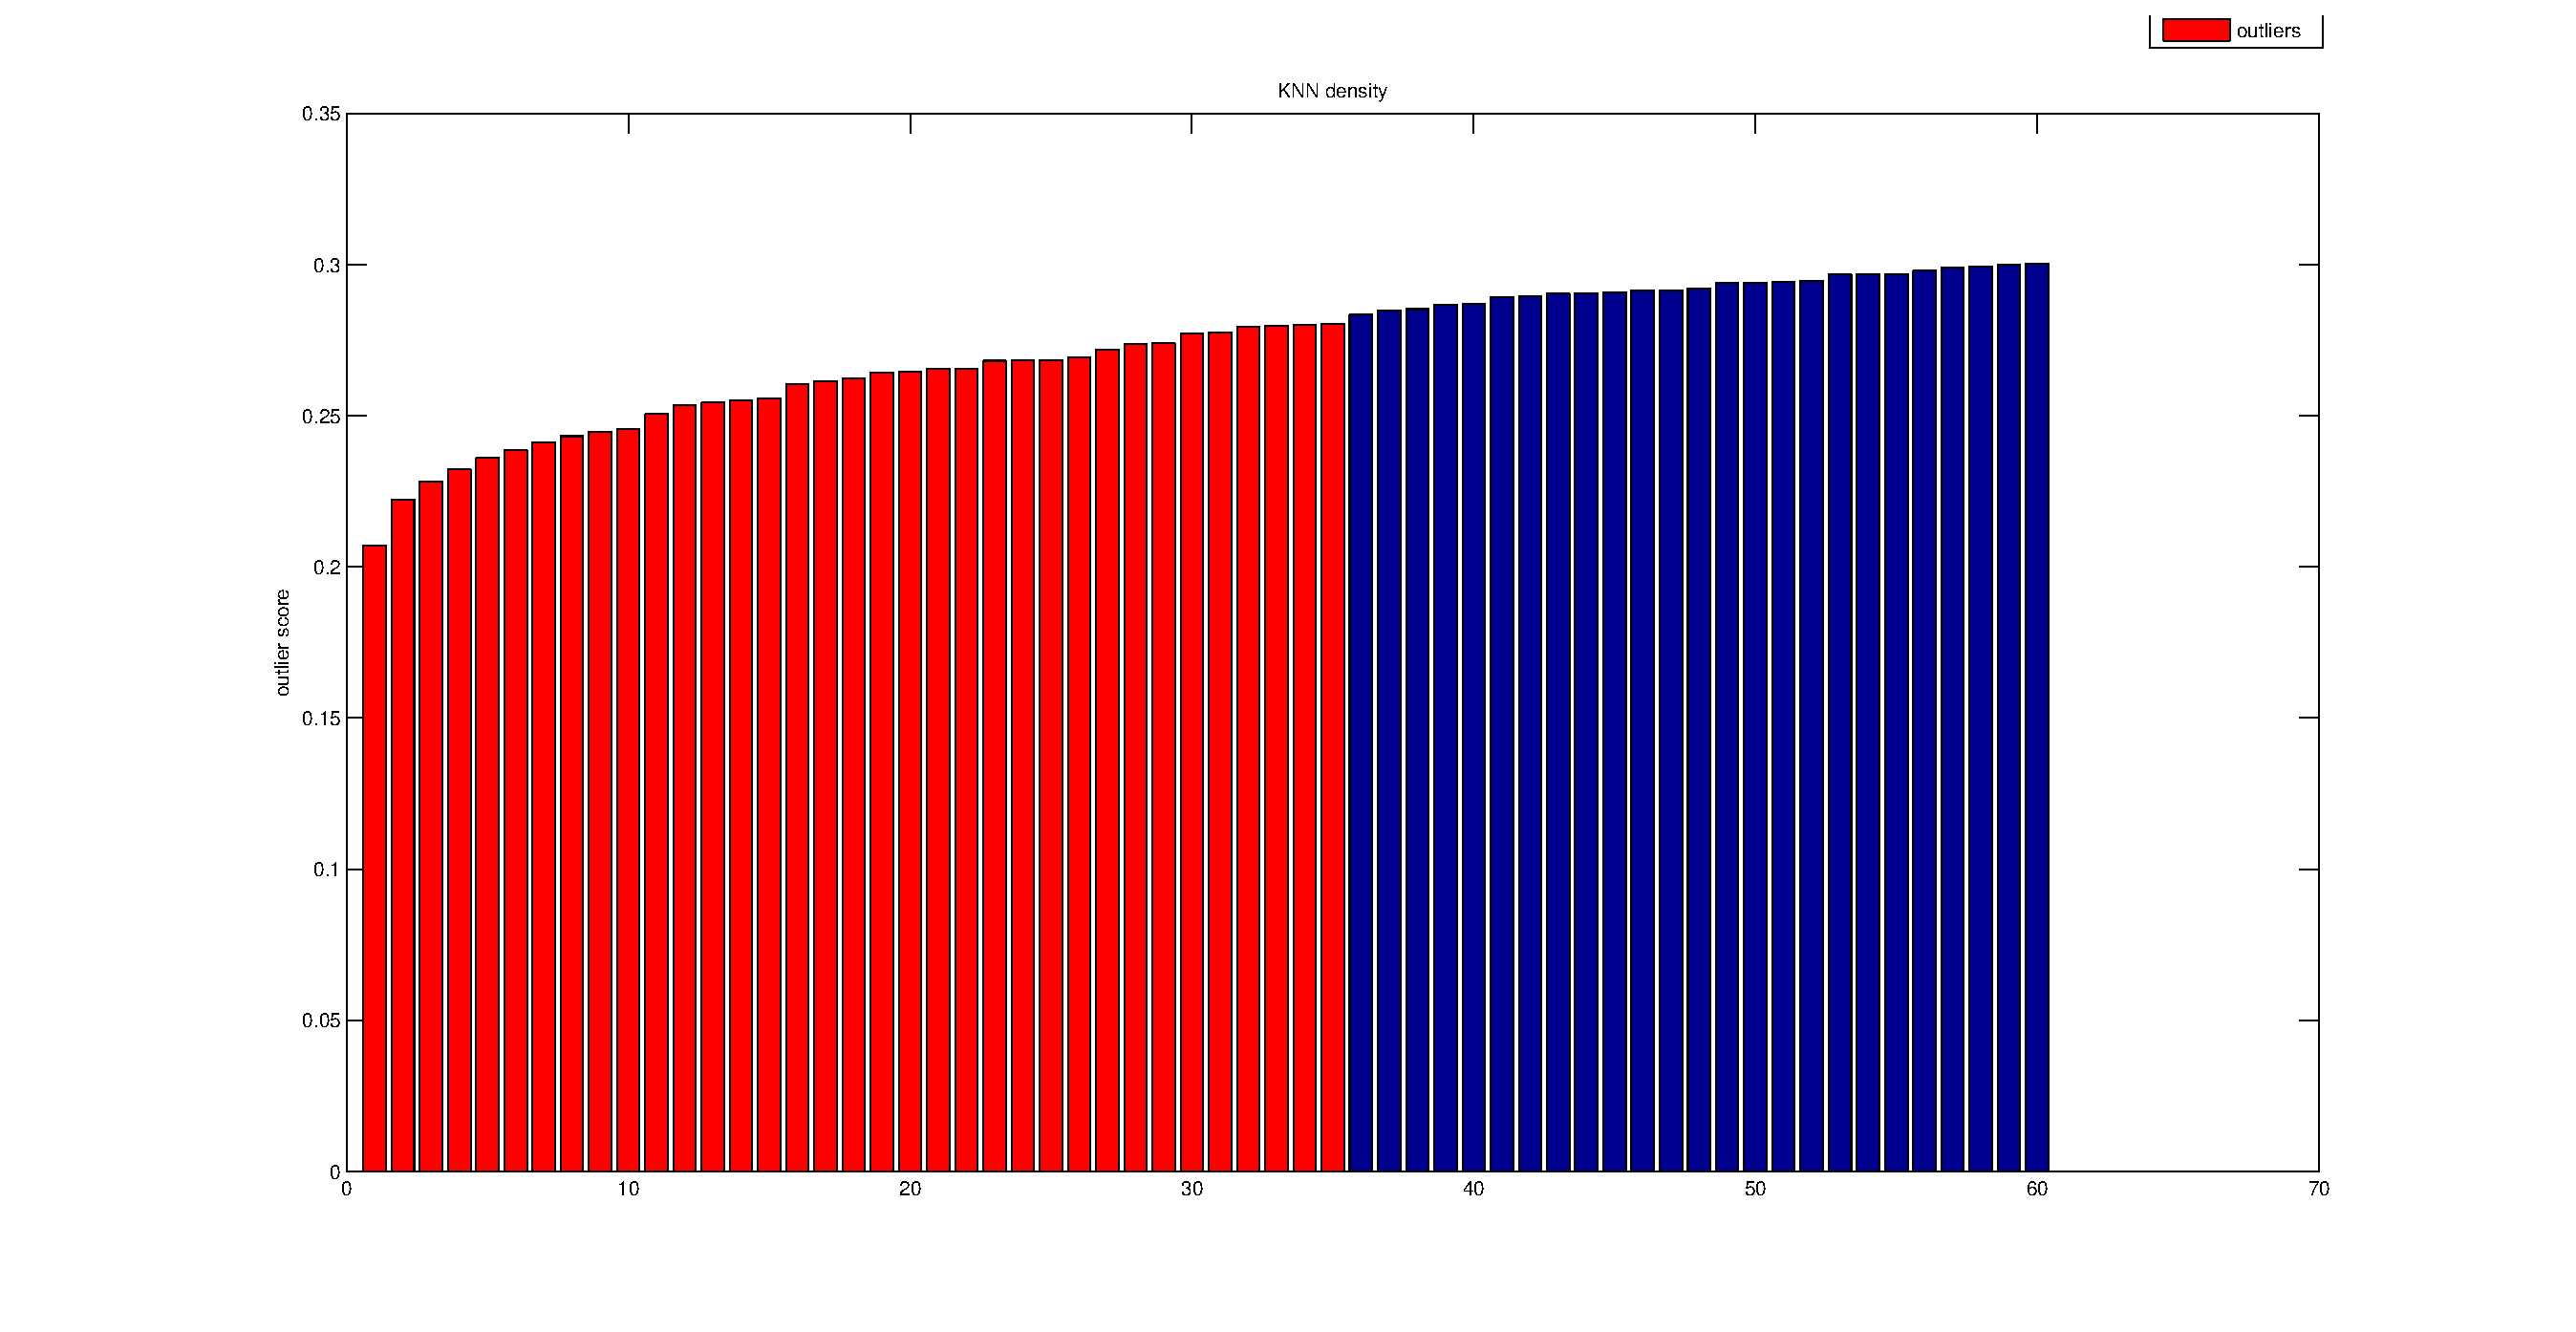
\includegraphics[width=7.4cm]{figures/02.eps}
                \caption{KNN density outliers}
         \end{subfigure} \\
	 \begin{subfigure}[b]{0.46\textwidth}
                 \linespread{1}
                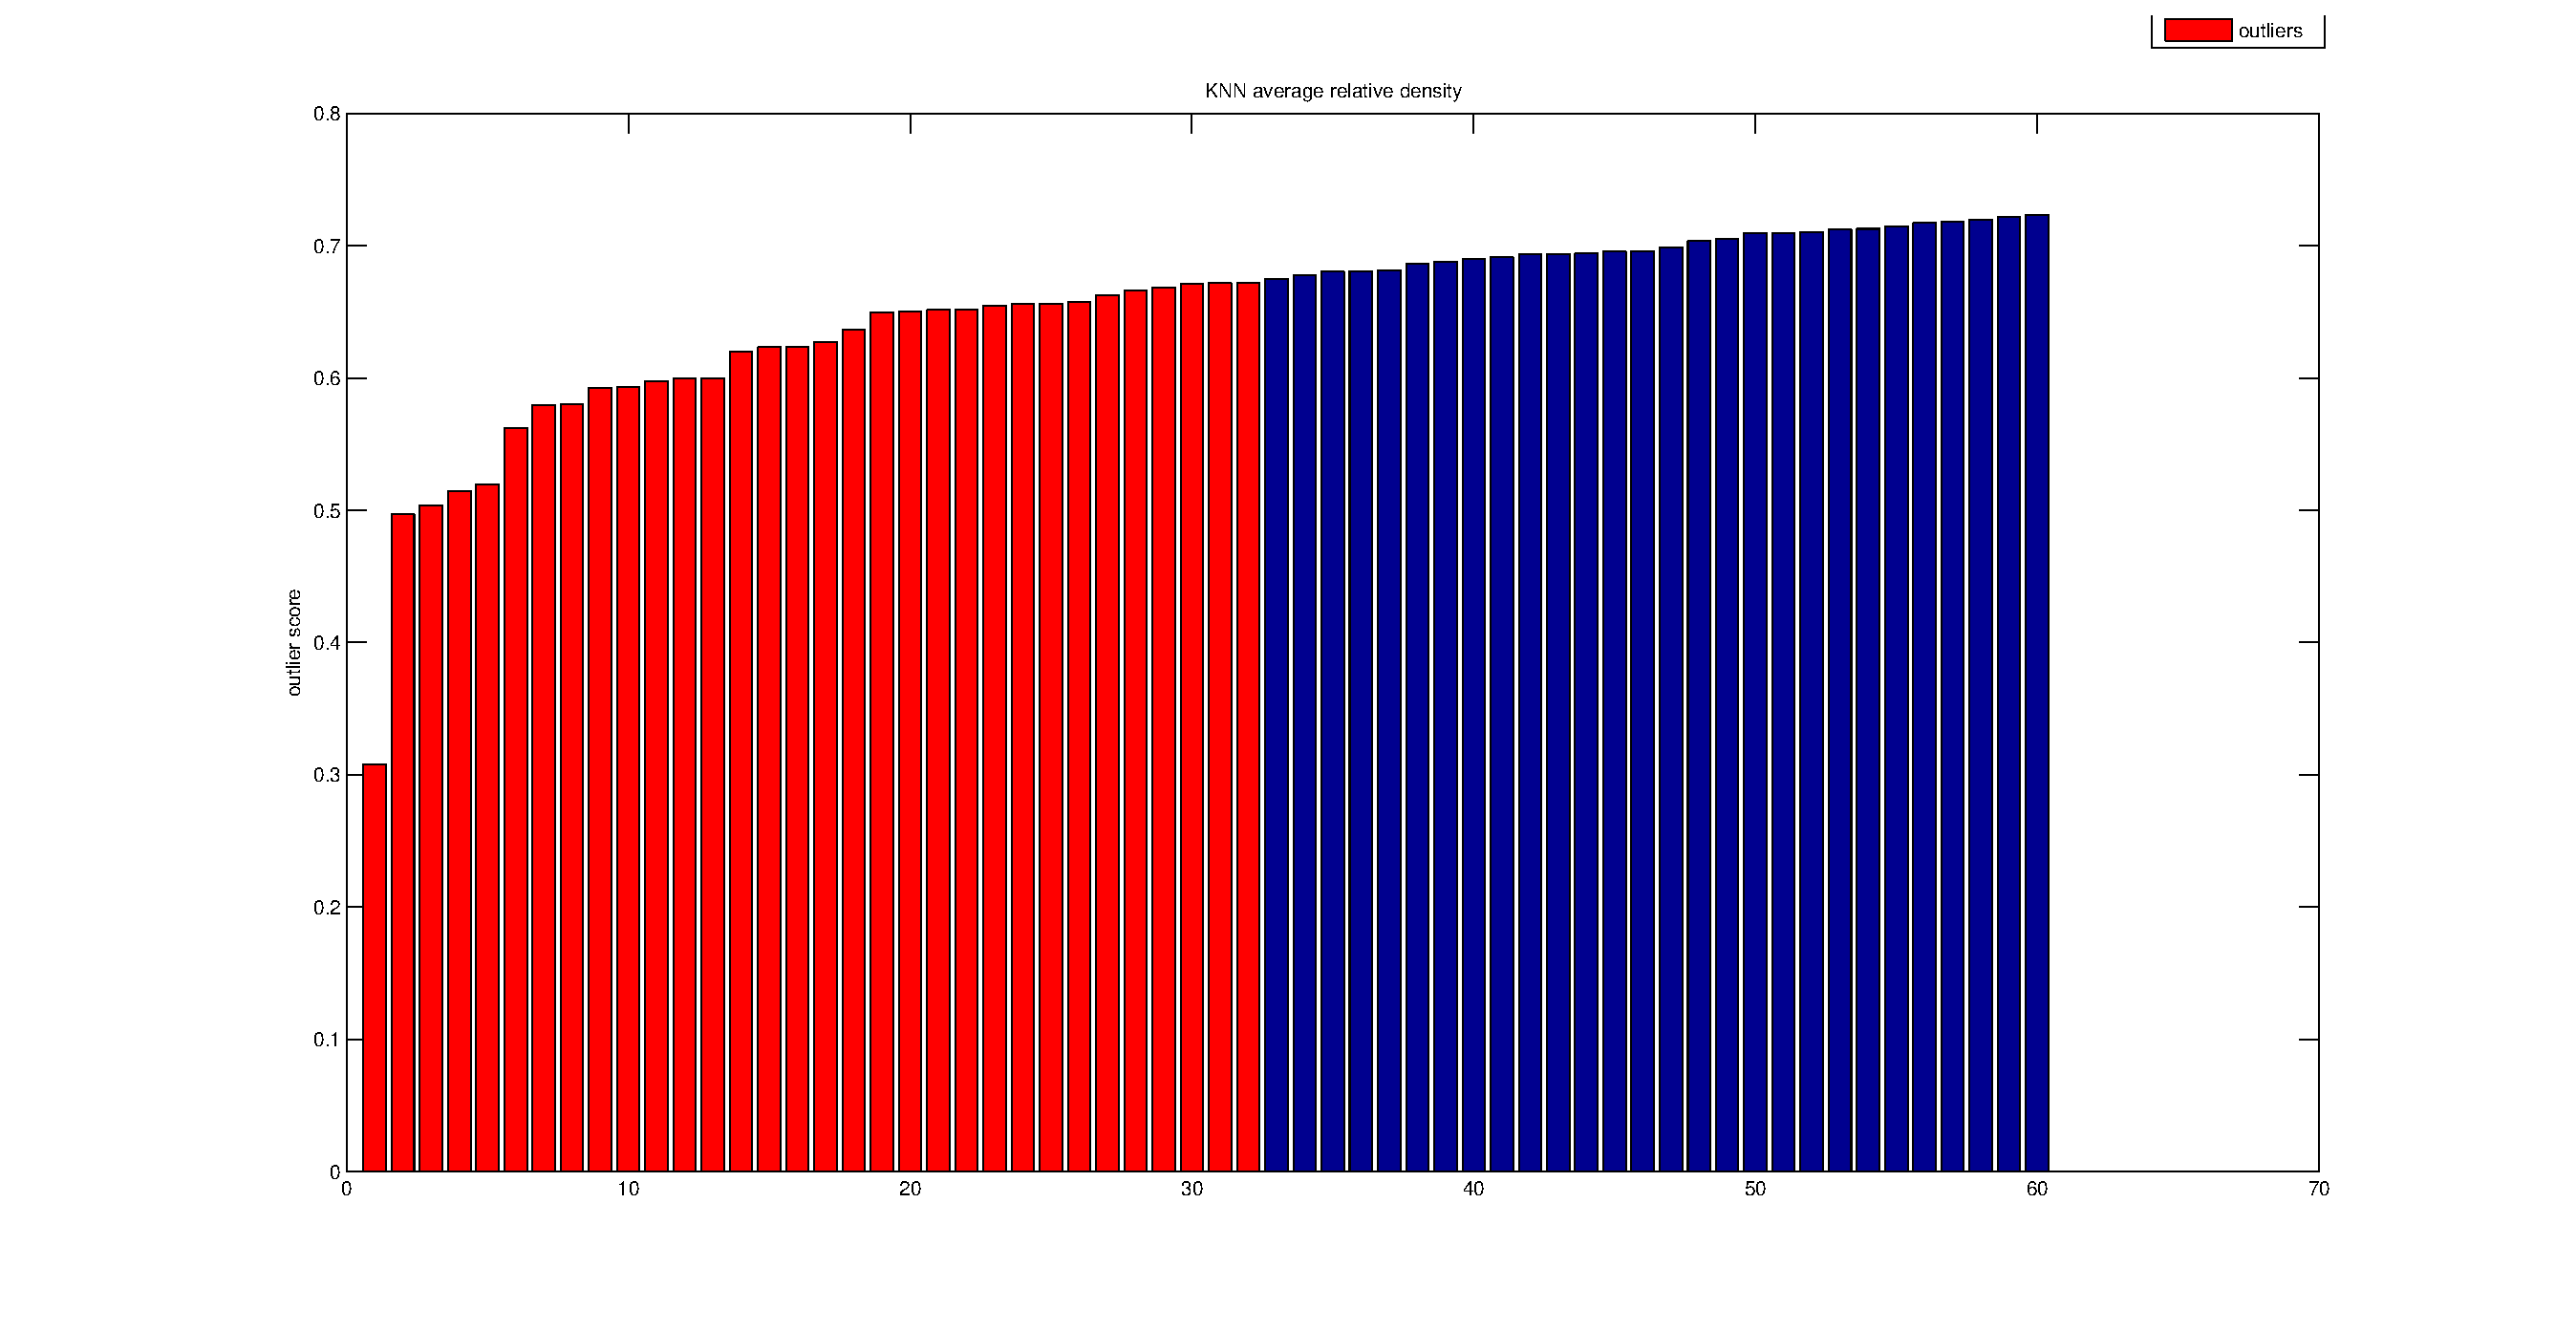
\includegraphics[width=7.4cm]{figures/03.eps}
                \caption{KNN avg rel. density outliers }
        \end{subfigure}
                \qquad
	\begin{subfigure}[b]{0.46\textwidth}
                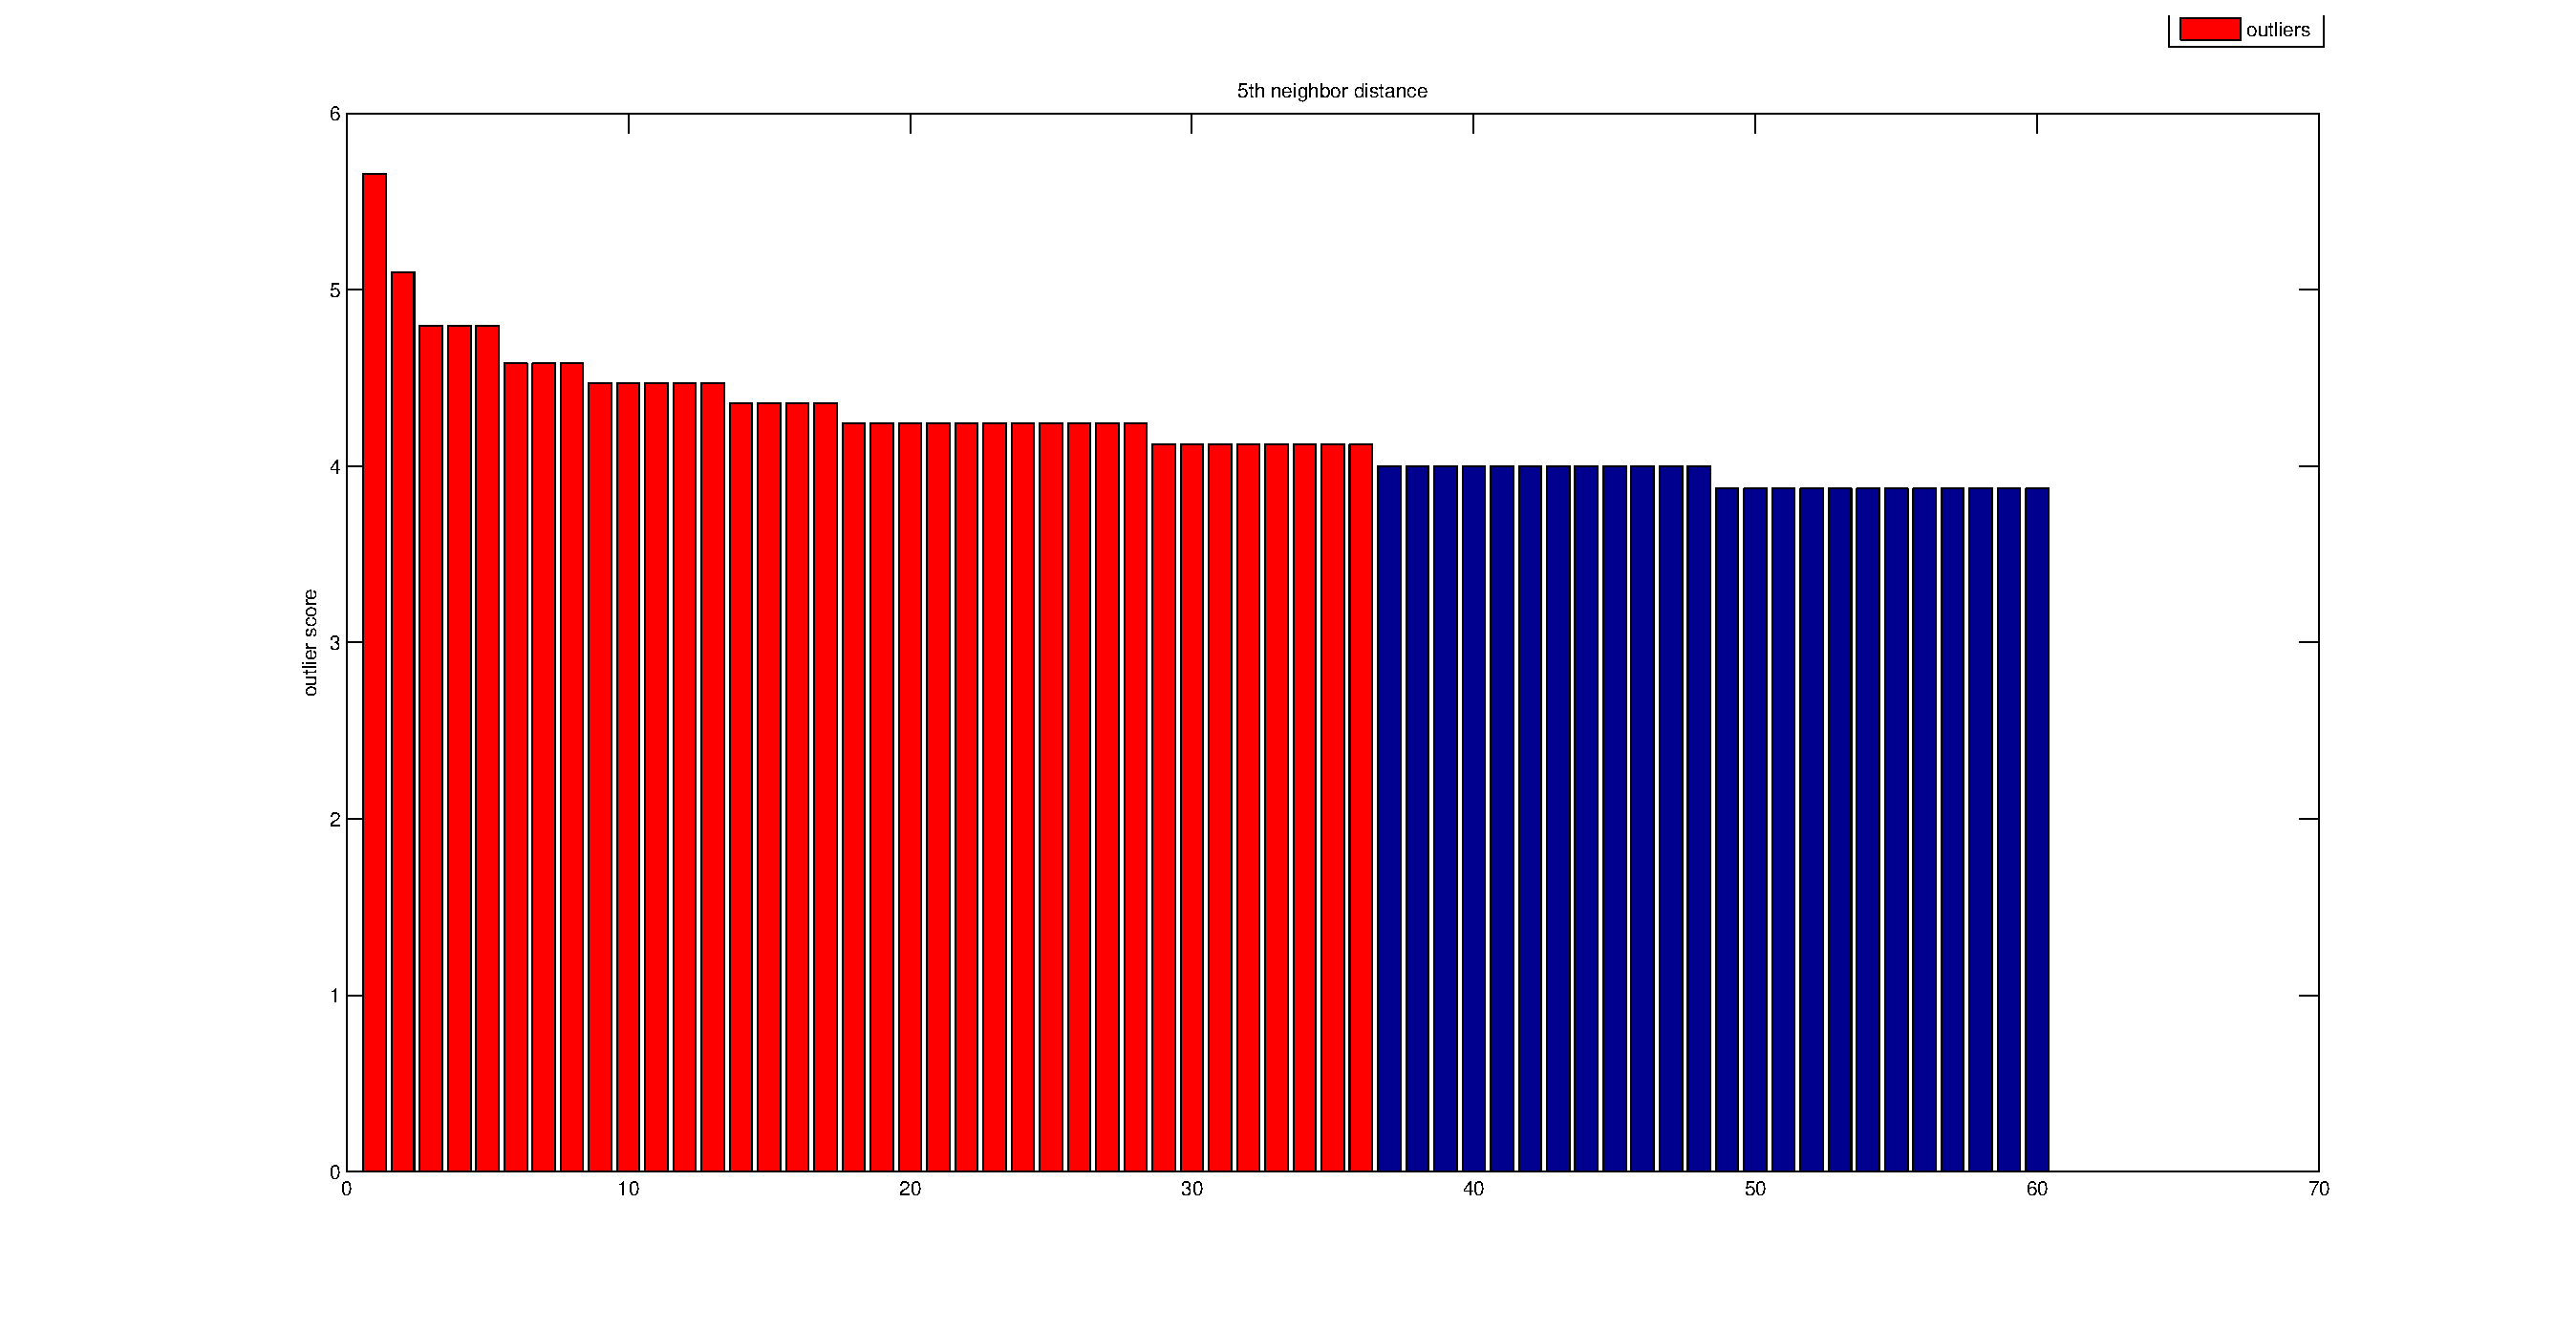
\includegraphics[width=7.4cm]{figures/04.eps}
                \caption{5th neighbor distance outliers}
         \end{subfigure} \\
        \caption{bar graph outliers}
         \label{fig:r1}
\end{figure}

To further understand the outliers distribution, for each scoring method we plot the outliers in the PCA space. Figures  \ref{fig:r2} shows that is not really possible to see a pattern for outliers in the PC1/PC2 space (maybe it could be possible find only few of them).
In figure \ref{fig:r3} you can see the outliers detected by all four methods.

\begin{figure}[htbp]
        \center
       	\begin{subfigure}[b]{0.55\textwidth}
                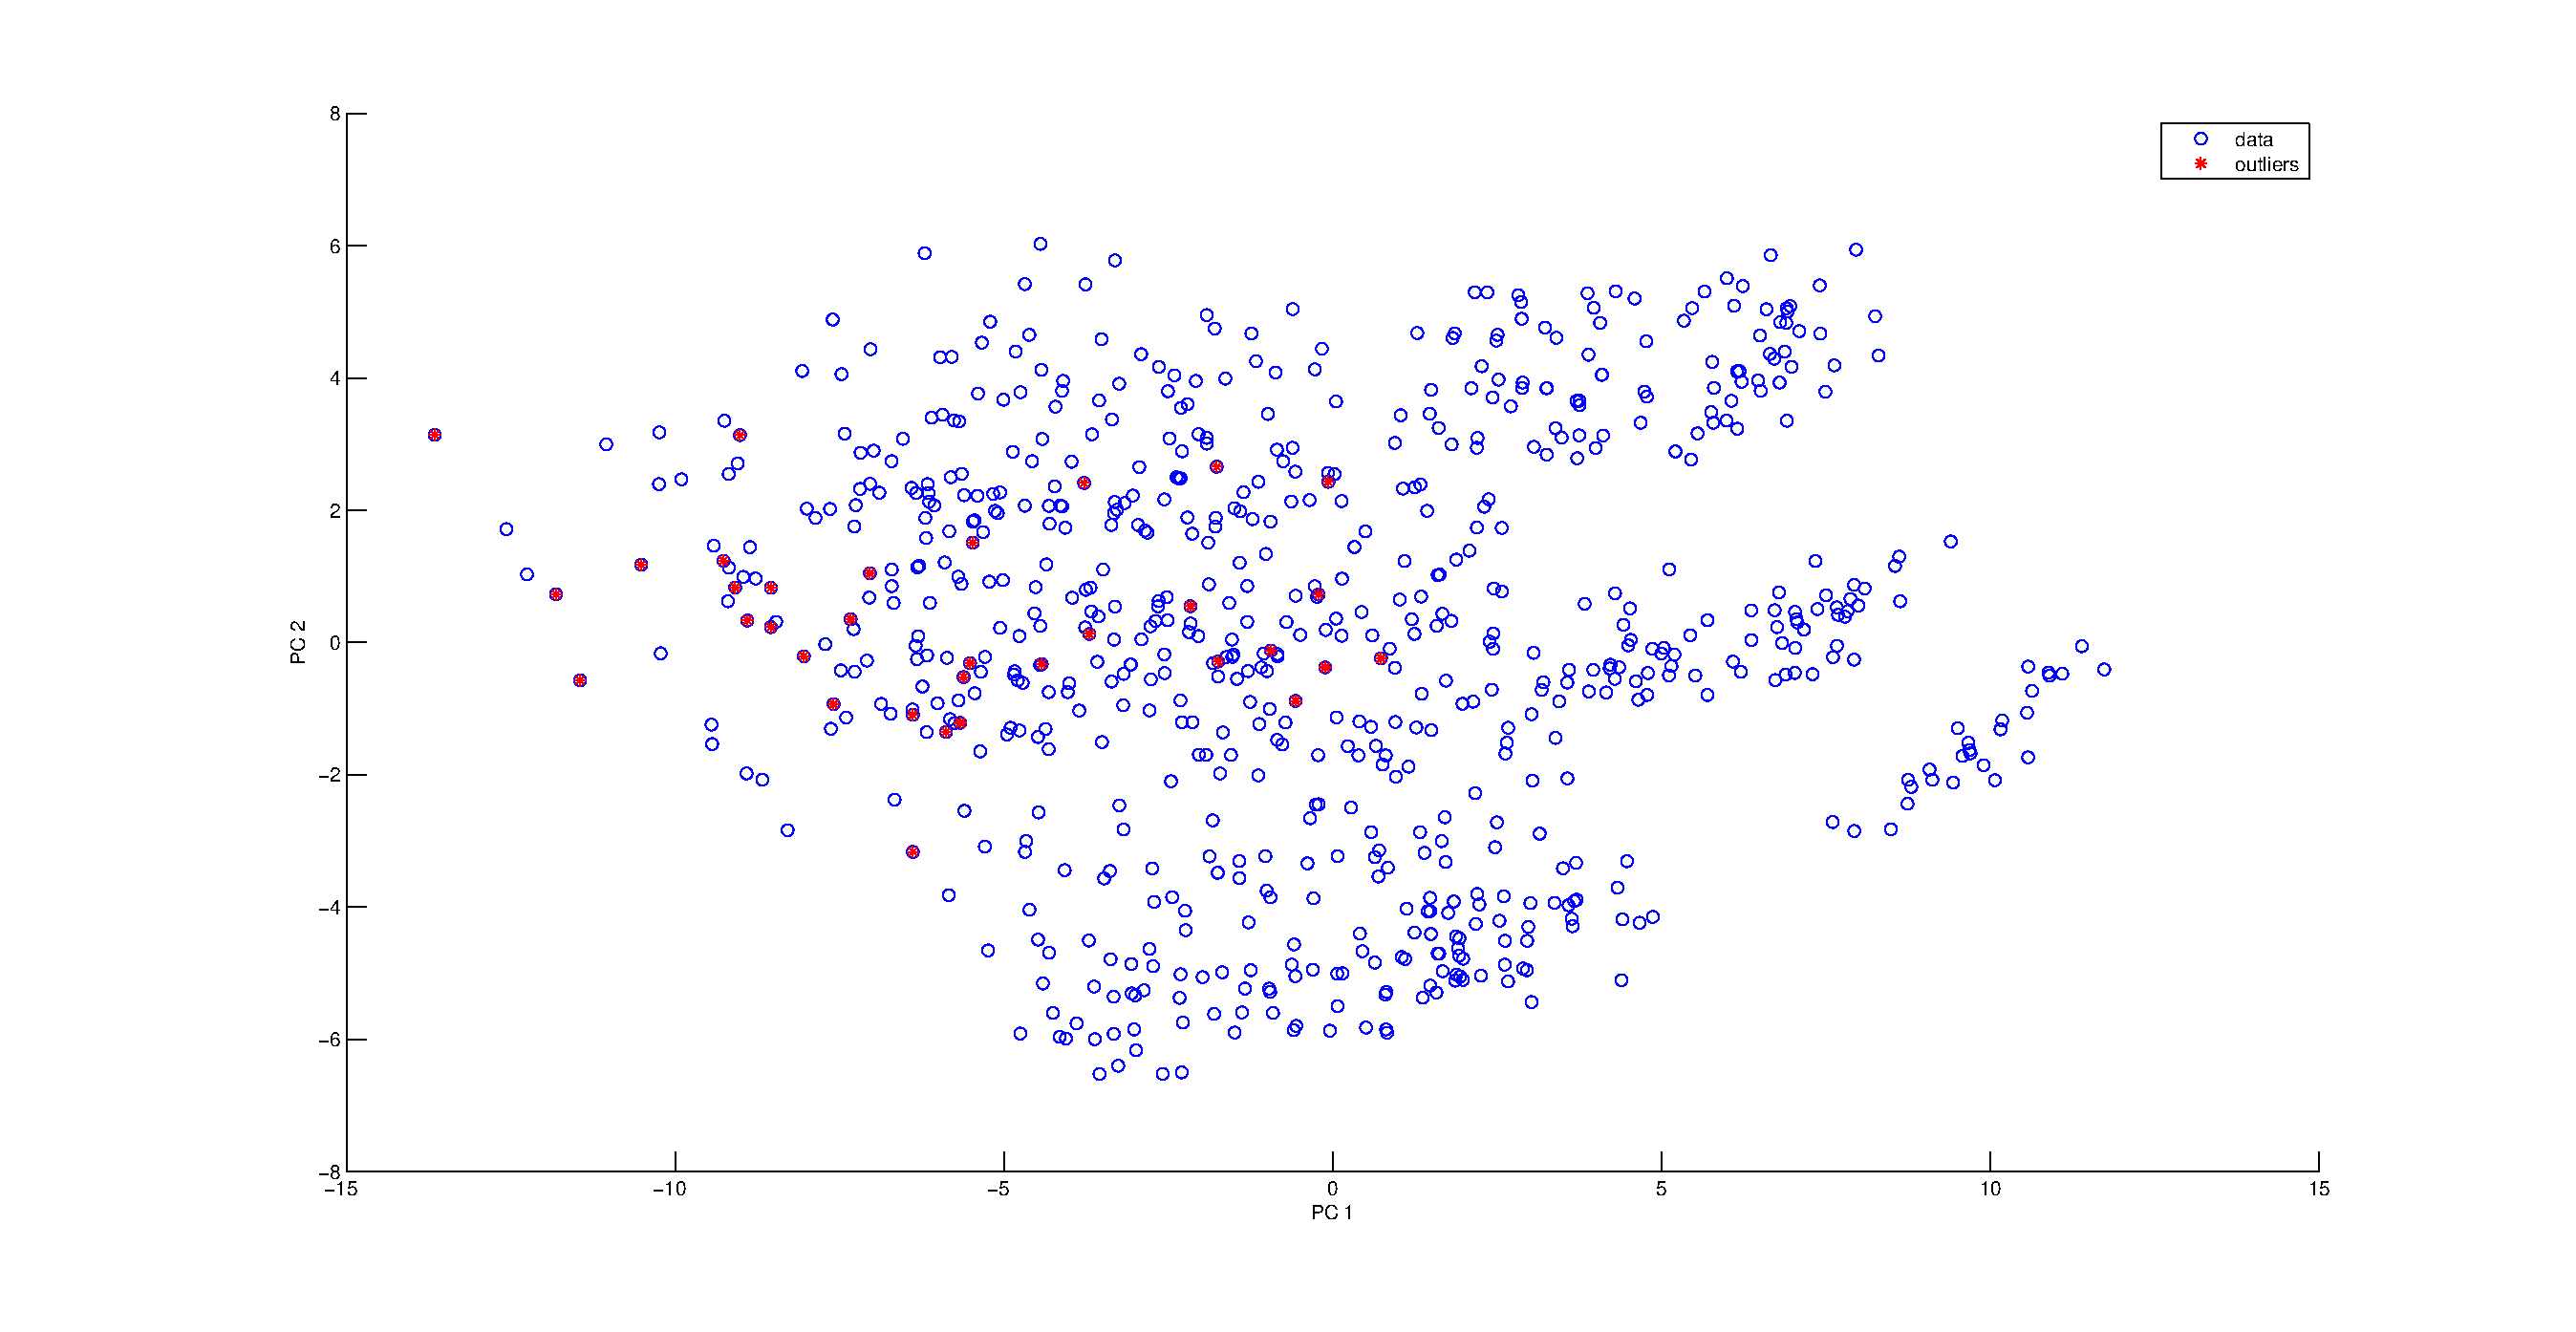
\includegraphics[width=10cm]{figures/pc1.eps}
                \caption{Density estimate outliers}
        \end{subfigure}%
        \quad
        \begin{subfigure}[b]{0.55\textwidth}
                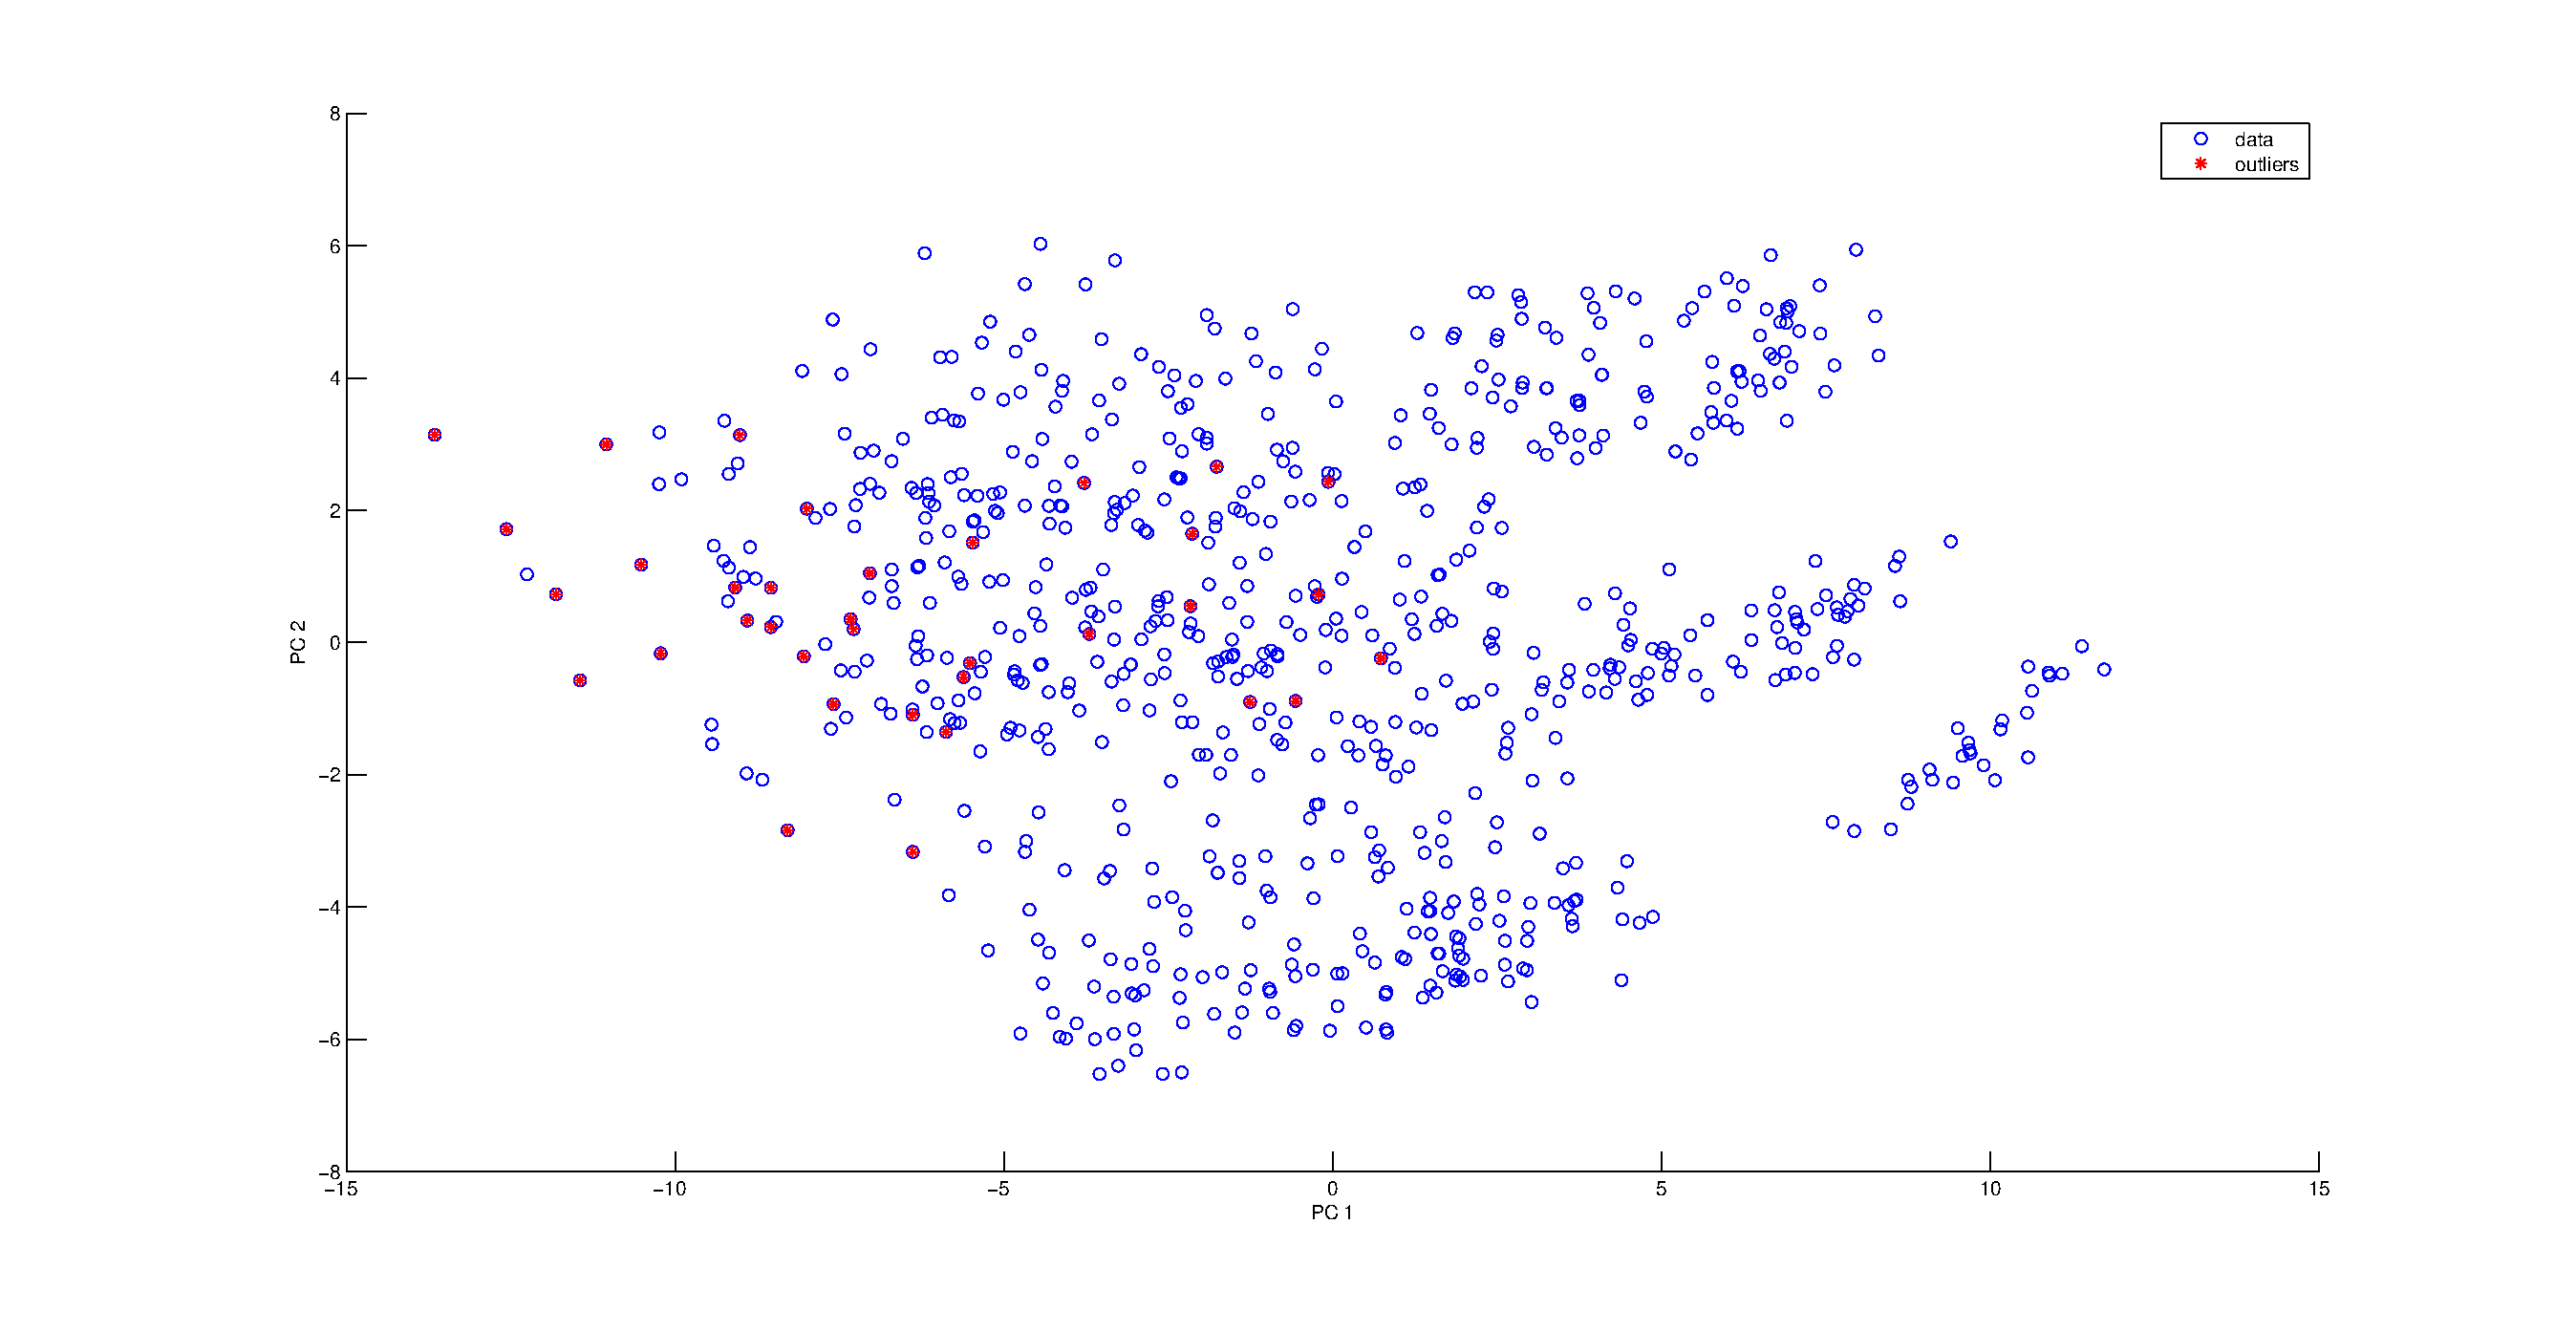
\includegraphics[width=10cm]{figures/pc2.eps}
                \caption{KNN density outliers}
         \end{subfigure} \\
	 \begin{subfigure}[b]{0.55\textwidth}
                 \linespread{1}
                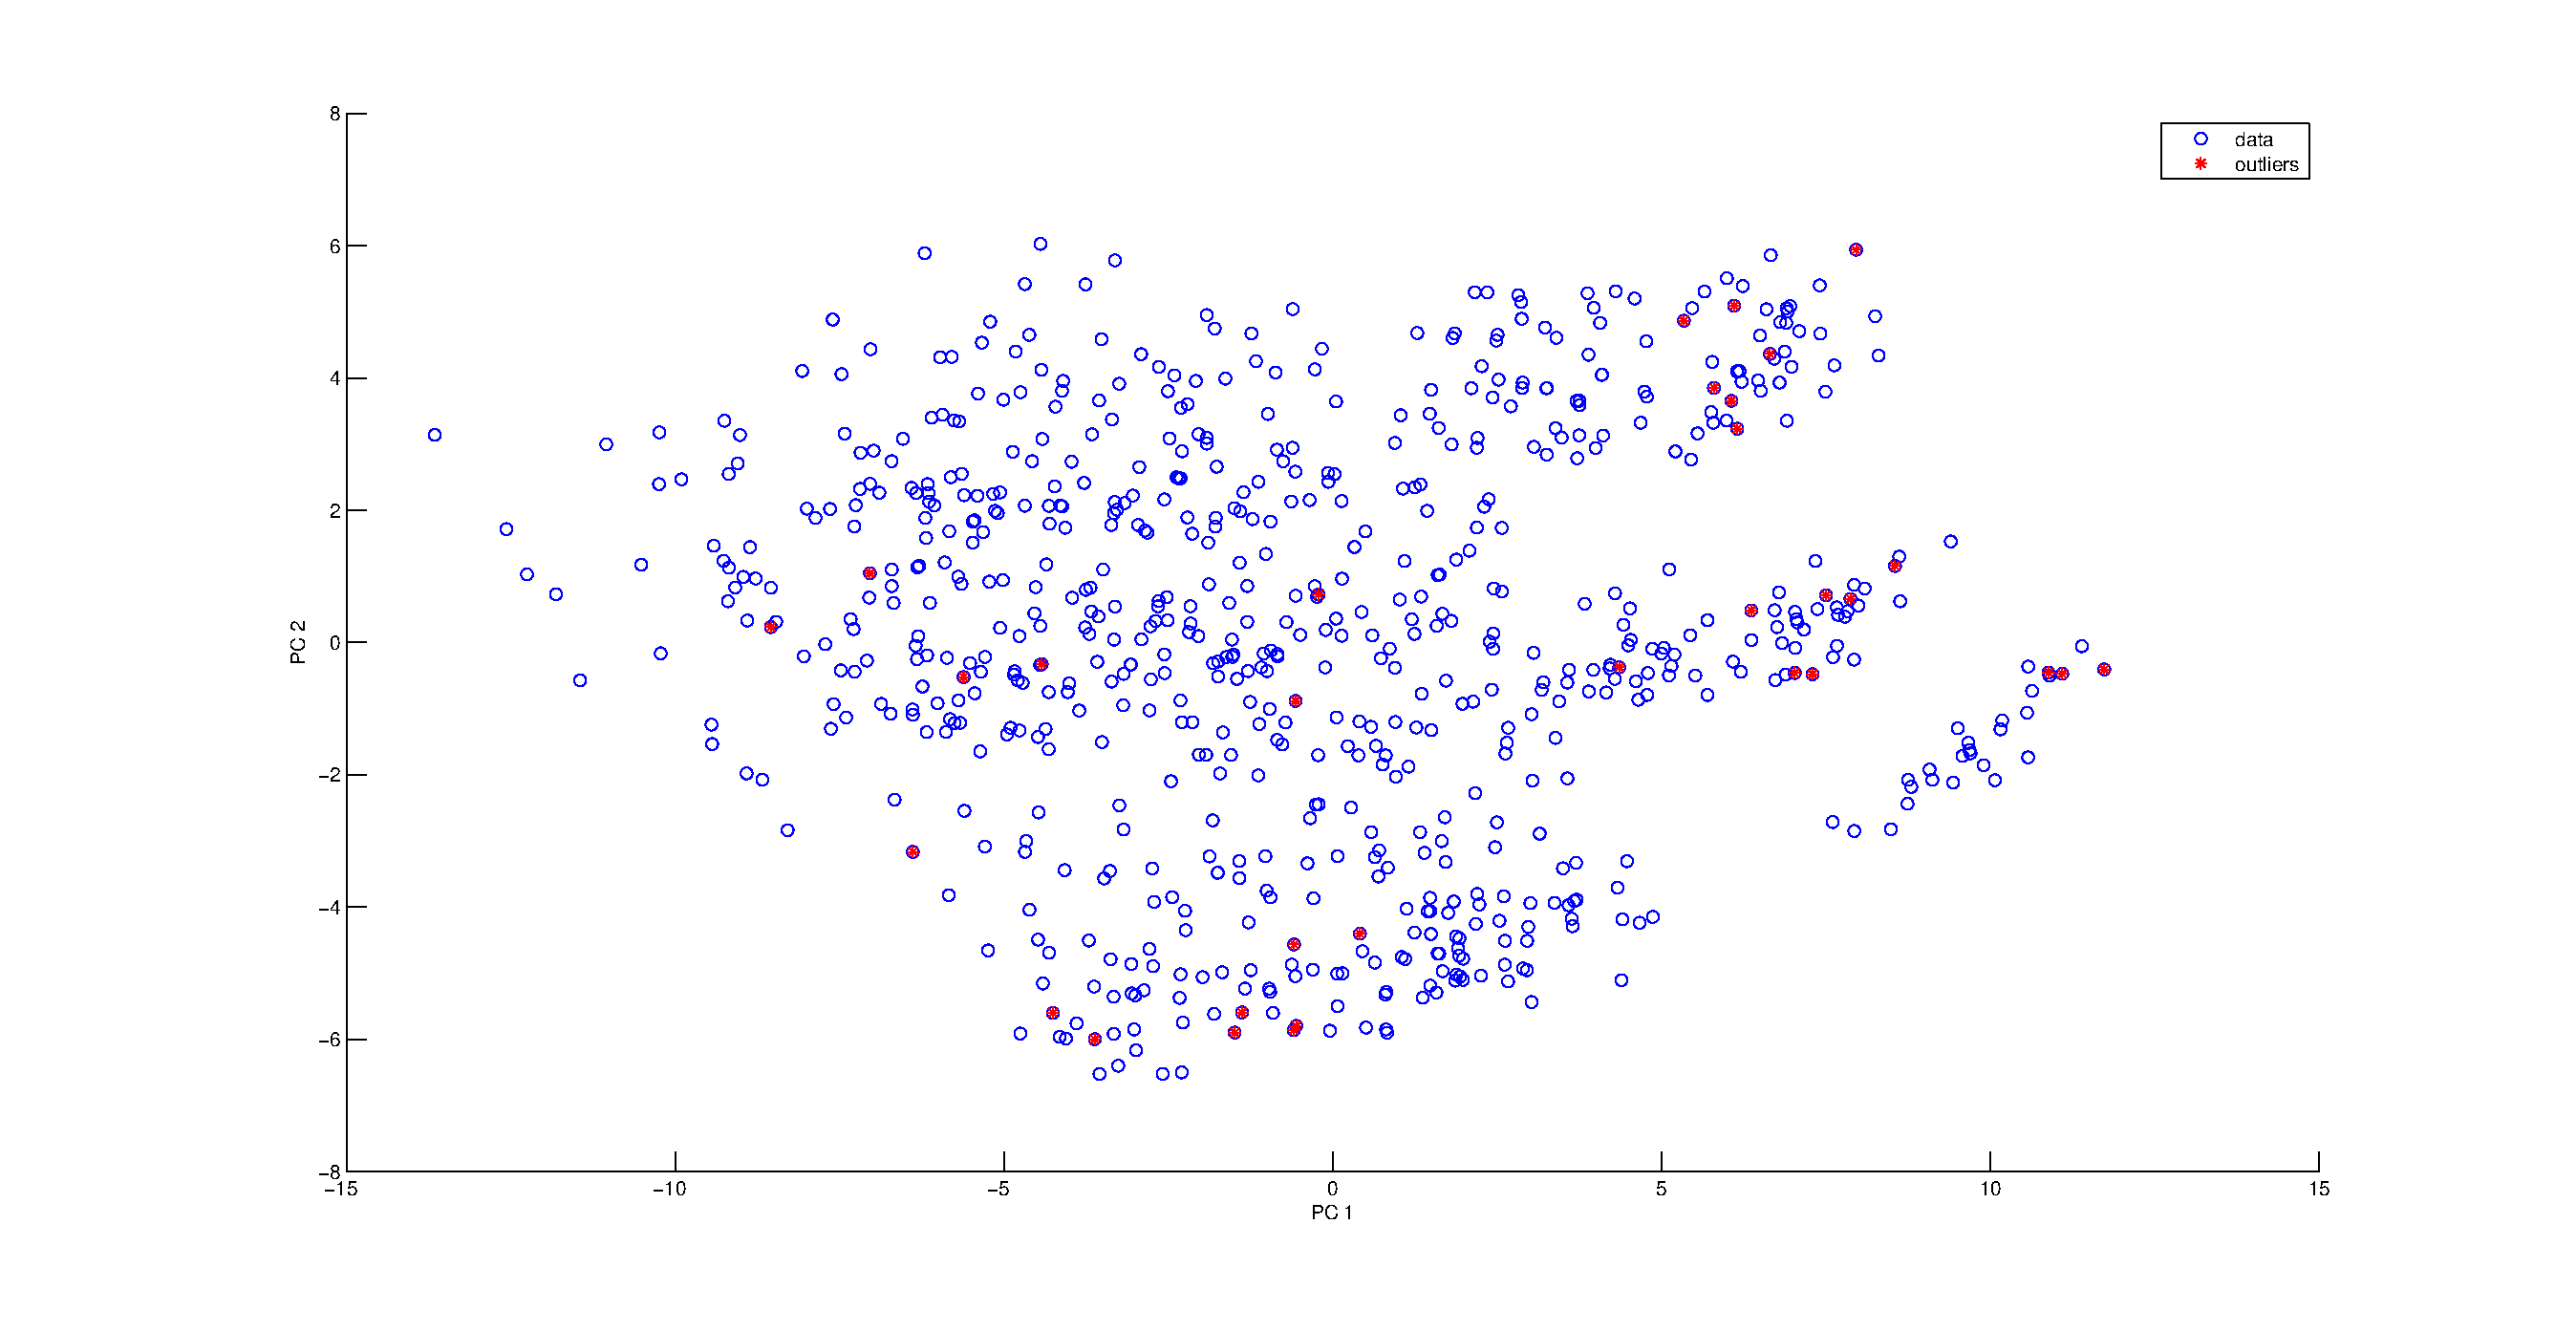
\includegraphics[width=10cm]{figures/pc3.eps}
                \caption{KNN average relative density outliers }
        \end{subfigure}
                \quad
	\begin{subfigure}[b]{0.55\textwidth}
                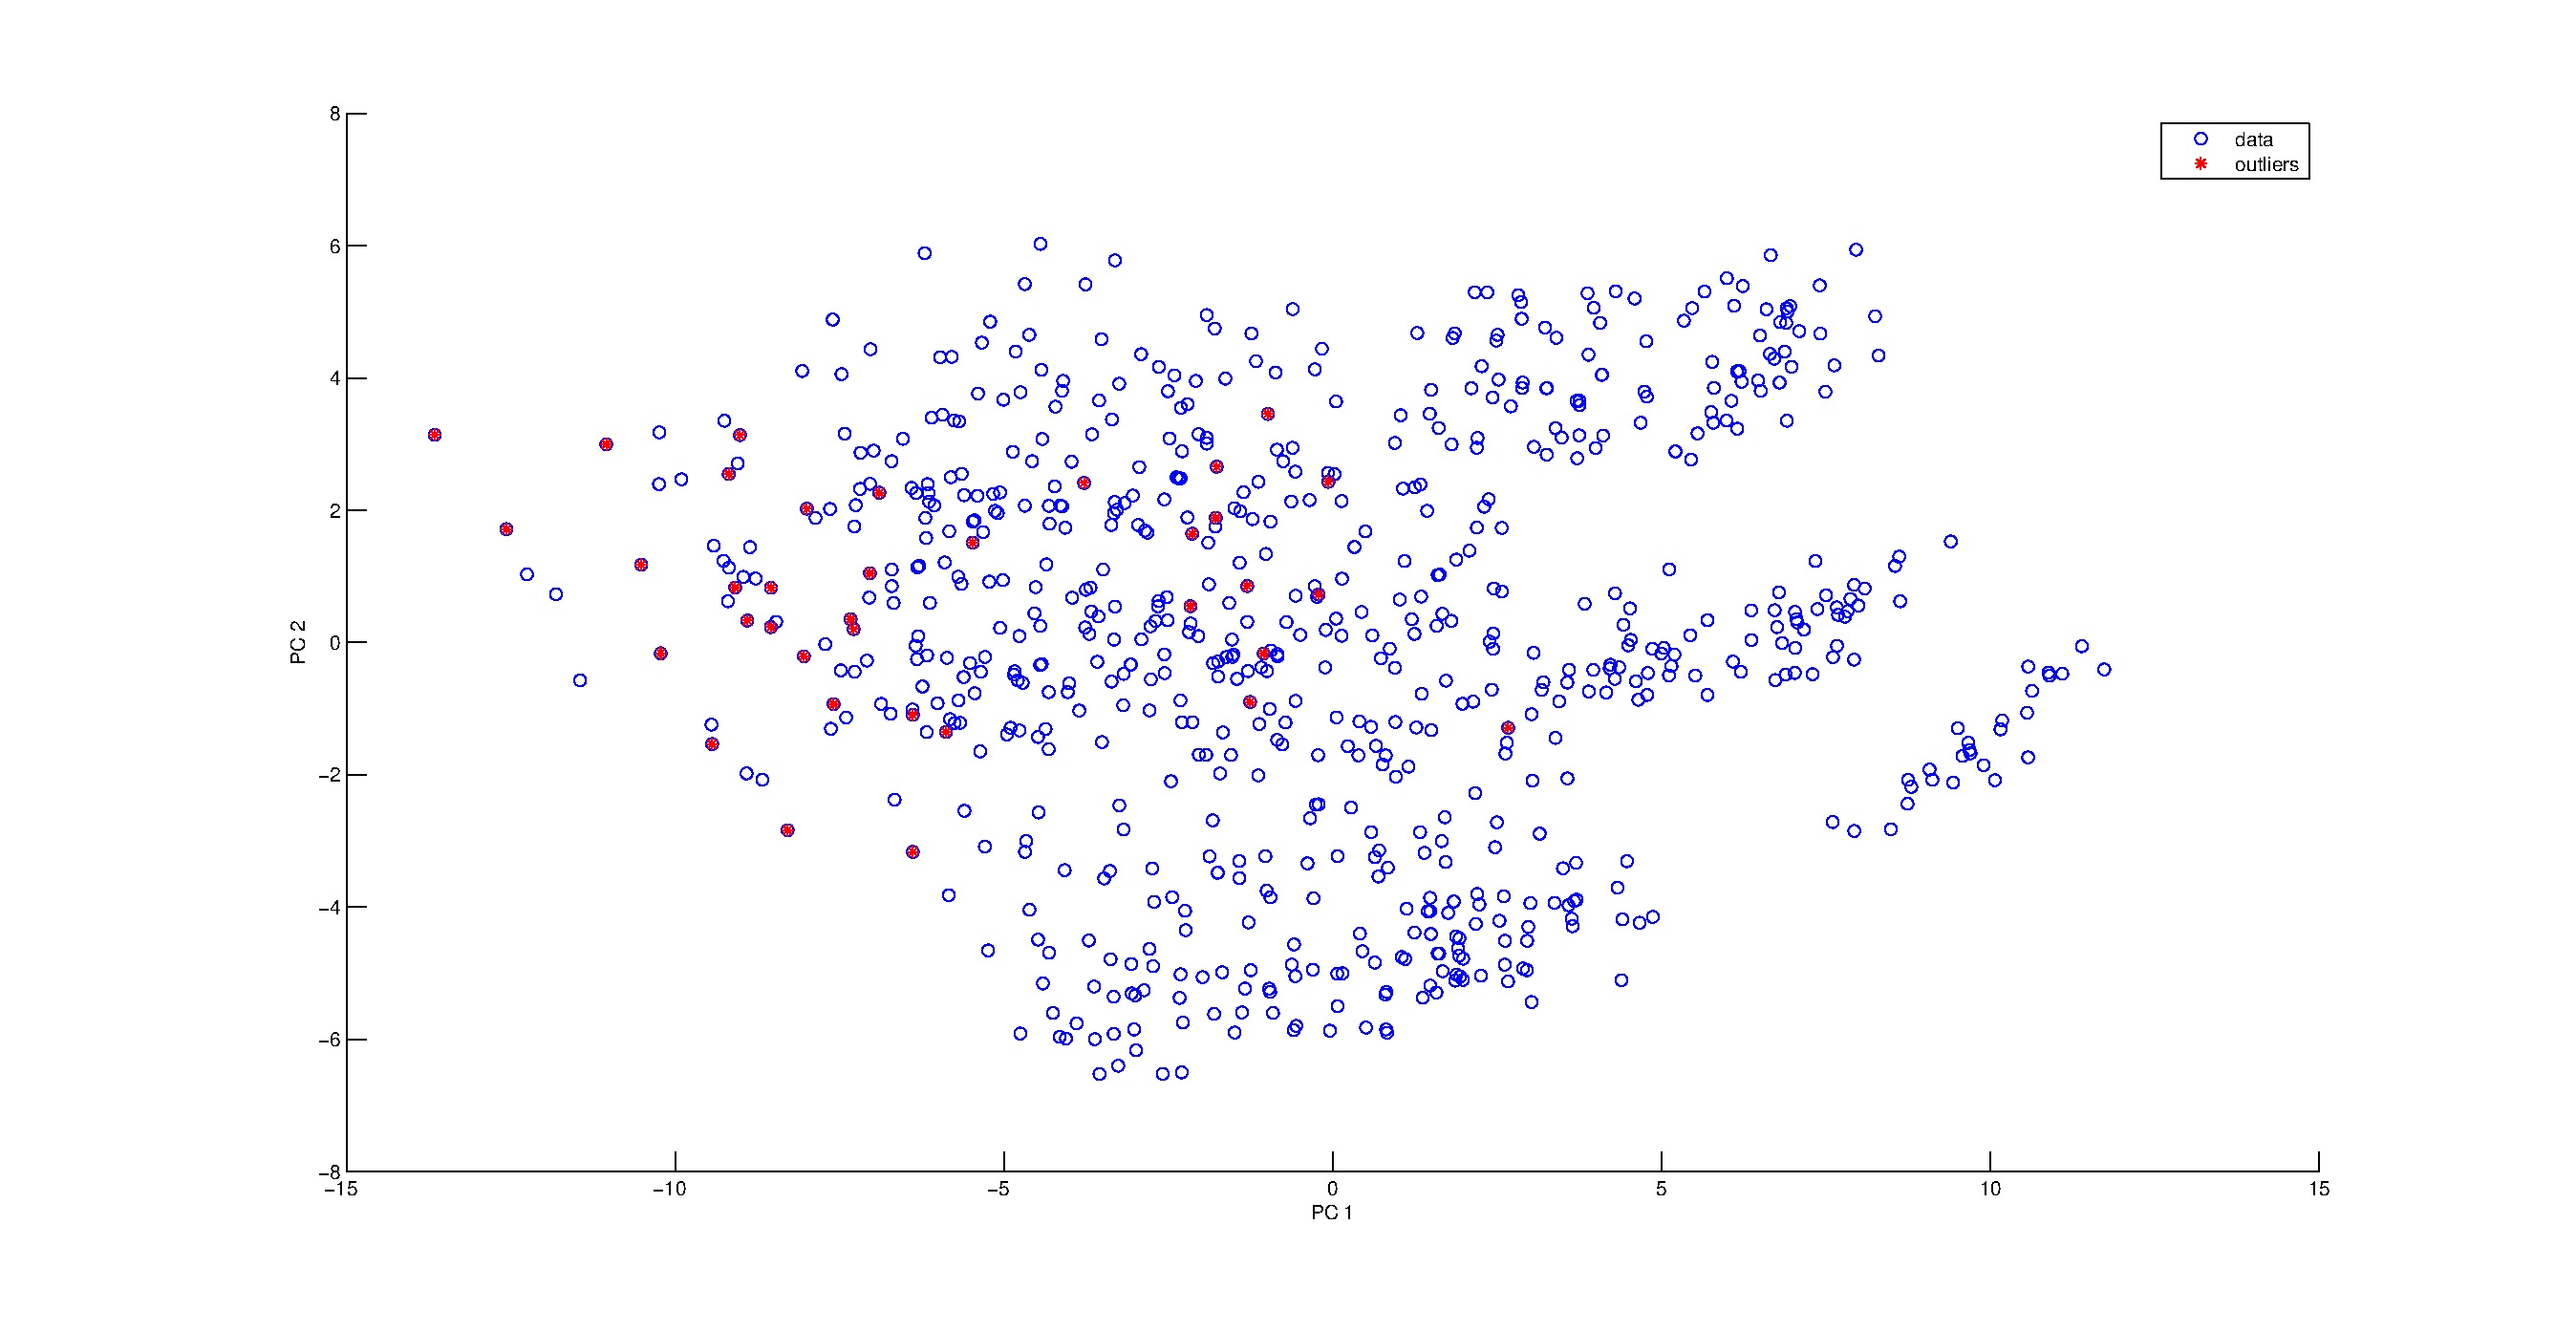
\includegraphics[width=10cm]{figures/pc4.eps}
                \caption{5th neighbor distance outliers}
         \end{subfigure} \\
        \caption{Principal component plot with outliers}
        \label{fig:r2}
\end{figure}

\begin{figure}[htbp]
        \center
                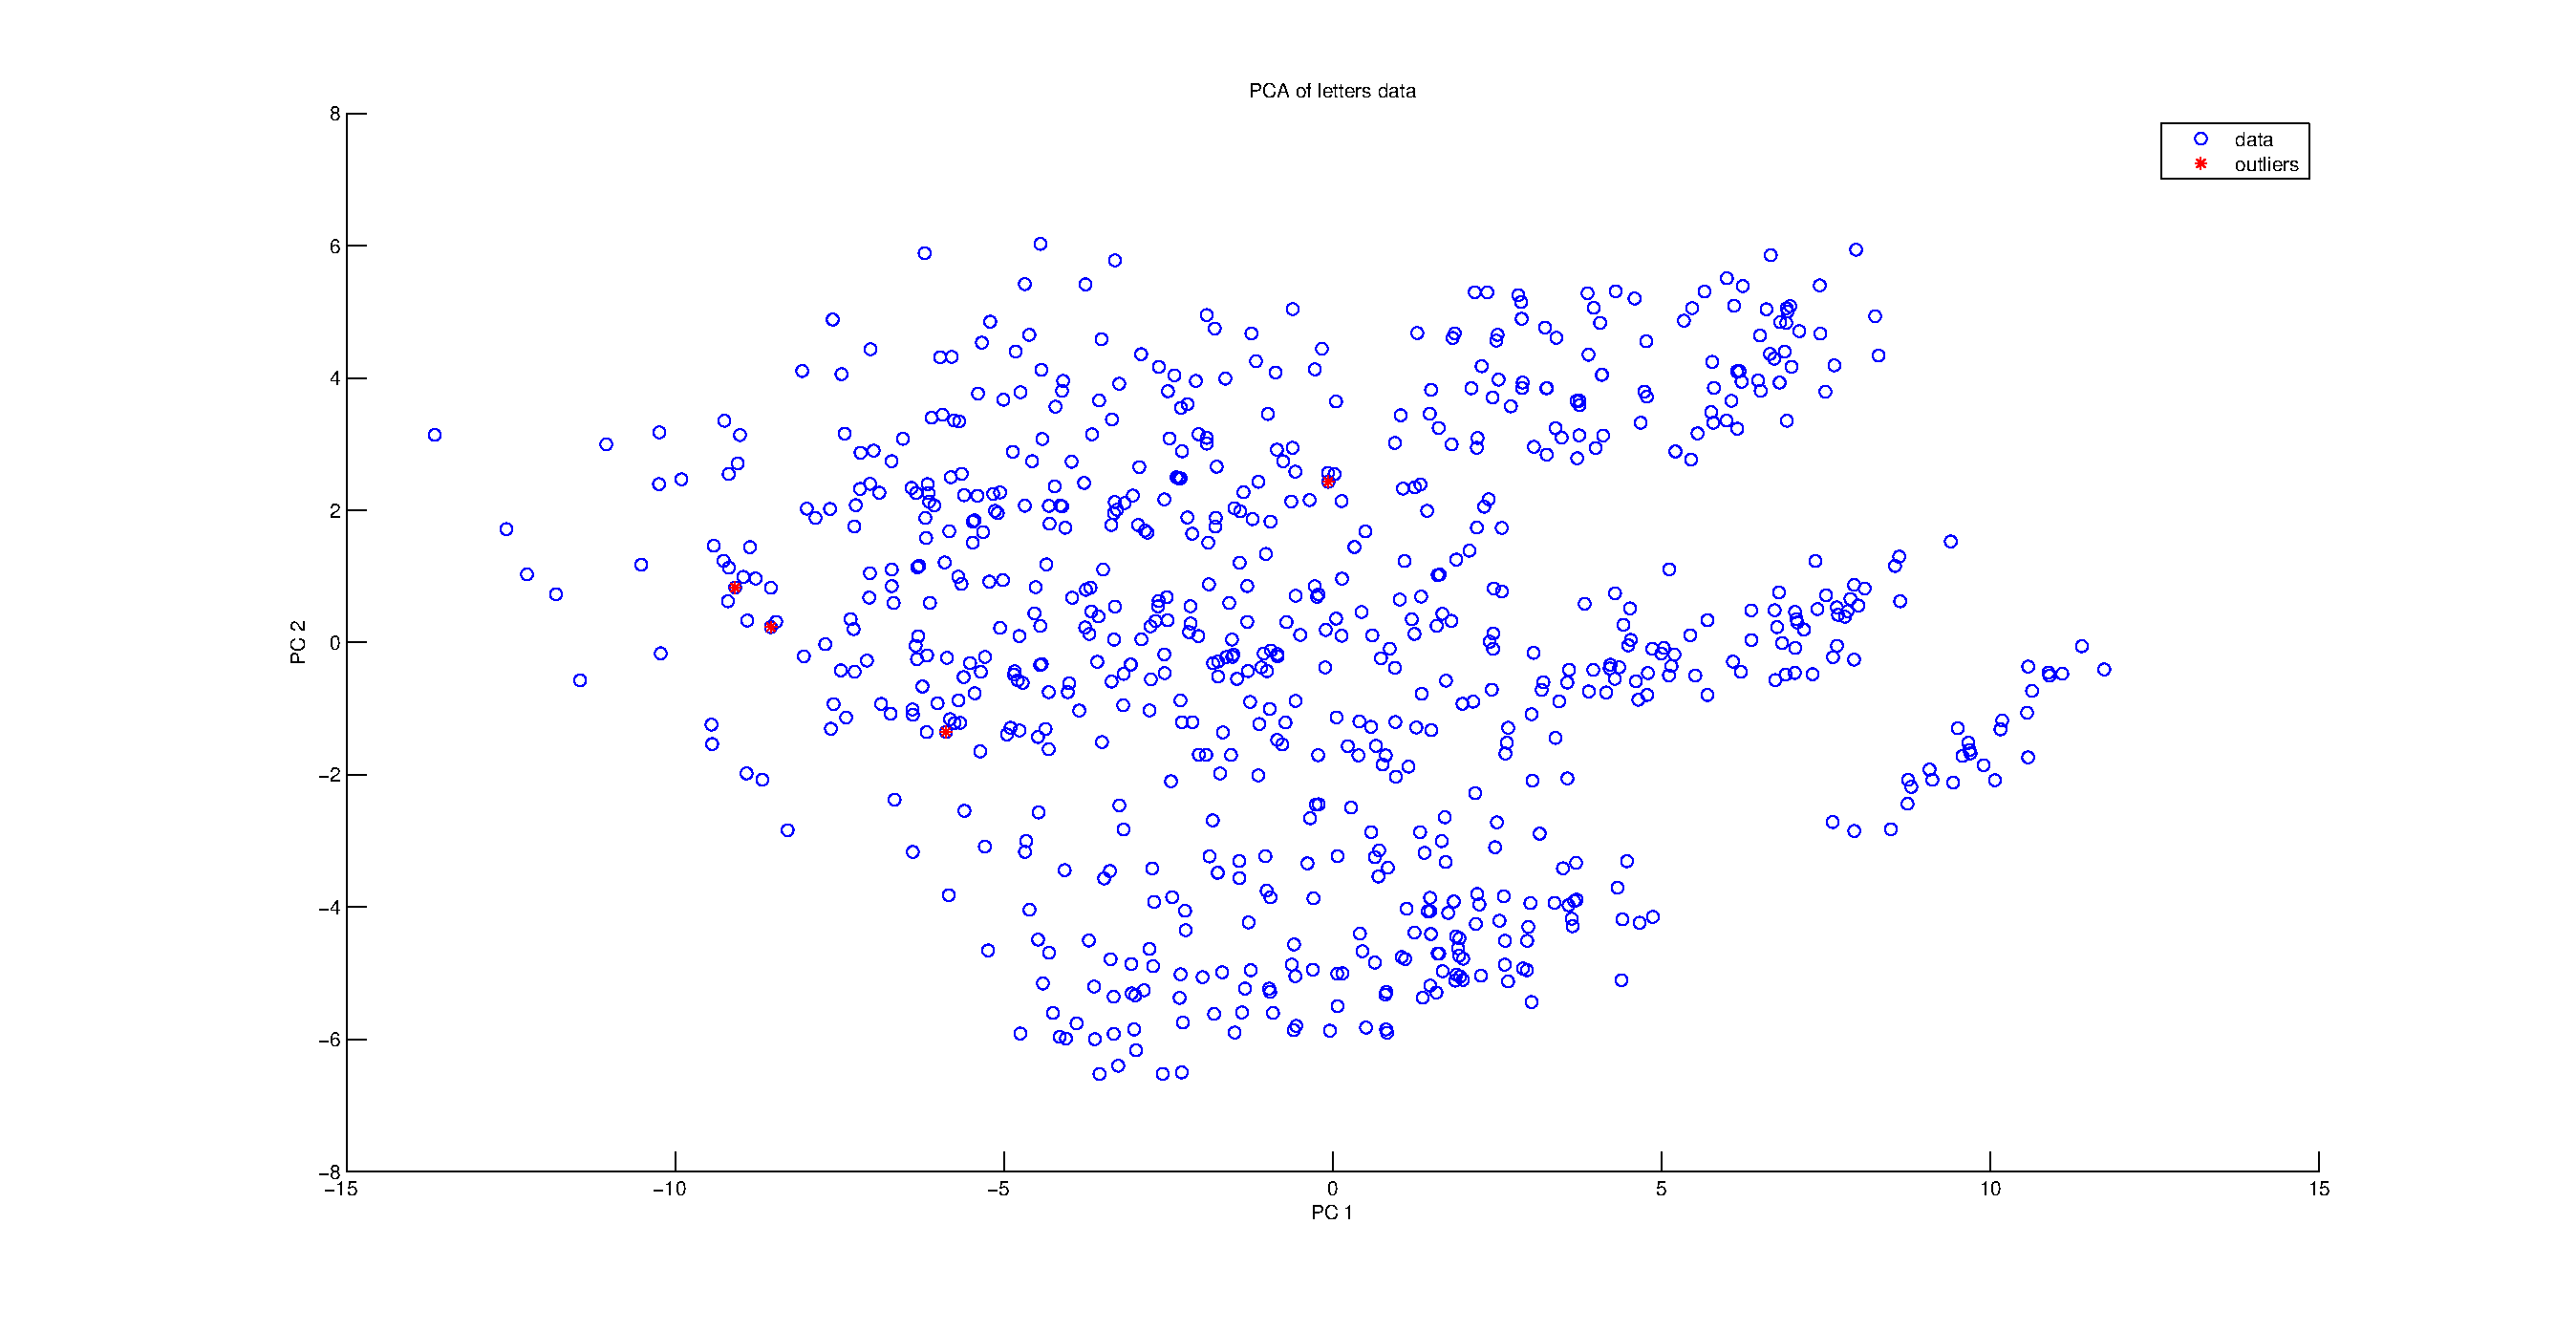
\includegraphics[width=10cm]{figures/pc5.eps}
                \caption{outliers detected by all four methods}
        \label{fig:r3}
\end{figure}


We applied outlier detection using different metrics, and by setting an appropriate threshold we identified some outliers, constituting about 0.5\% of our dataset. Anyway we are never sure whether a certain pattern is an outlier but we can just suppose it especially because we have a wide dataset so is probable that some patterns are distant from other observations.
\end{document}
\chapter*{Conclusions}
Summing up our work, we observed that K-Nearest Neighbors algorithm is the best method for letter
classification on our dataset. Neural networks also gained good results, however they could be made
more precise applying deep neural networks with doing computations on GPU. Some of our methods
were a way better than these presented by previous researchers. 

%\chapter*{Preface} 
Preface text\dots

%\chapter{Testing}
\section{Images}
Always have images/figures in \emph{both} EPS and PDF/PNG/JPG format! (unless you know you only will be using pdfLaTeX)


\begin{figure}[!tbh]
	\centering
	
\includegraphics[width=0.5\textwidth]{testimage}
	\caption{Test of image insertion.}
	\label{fig:testimage}
\end{figure}

\section{Tables}
\begin{table}[!h]
\centering%
\caption{Simple table.}\label{tab:table}
\begin{tabular}{| r l |}
   \hline
   aaaaaaaaaaaaaaa & bbbbbbbbbbbbb\\
   c & d\\
   \hline
\end{tabular}
\end{table}

\section{References} References are made with `\ref{tab:table}'. Refer to a page with 
`\pageref{tab:tabel}'.

\section{Bibliography} \cite{Deitel:2002} is a reference to a book.
%\bibliographystyle{plain} % pr�v ogs�: is-unsrt, alpha, plain
\bibliography{biblio/template-bib}
%\nocite{*} % \nocite bruges til b�ger som skal med i litteraturlisten
            % men som ikke er refereret til. Alts� baggrundsstof mv.


%\appendix % Alphabetic chapter numbering
%\renewcommand{\appendixtocname}{Appendix} % Change appendix name for the table od contents
%\addappheadtotoc % 'Appendix' to the table of contents
%\chapter{Appendix}
Insert your appendix here.
%\backmatter % for glossary, index, back page
\end{document}
